\section{Data to Monte Carlo comparisons at $\sqrt{s}=900$ GeV in
  Minimum Bias events}
\label{sc:DataVsMCMB900}

In this section we present the comparison of several calorimeter-based
distributions in data with {\sc pythia} Mininimum Bias Monte Carlo simulation. All distributions
shown in this section are required to pass the event selections
described in Sec.4. The Monte Carlo distributions shown in this section
are normalized so that the total number of events in Monte Carlo sample
mathces the number of events observed in data.


\subsection{Basic $\etmiss$-related distributions}
\begin{figure}[h!]
 \centering
 \begin{tabular}{ll}
  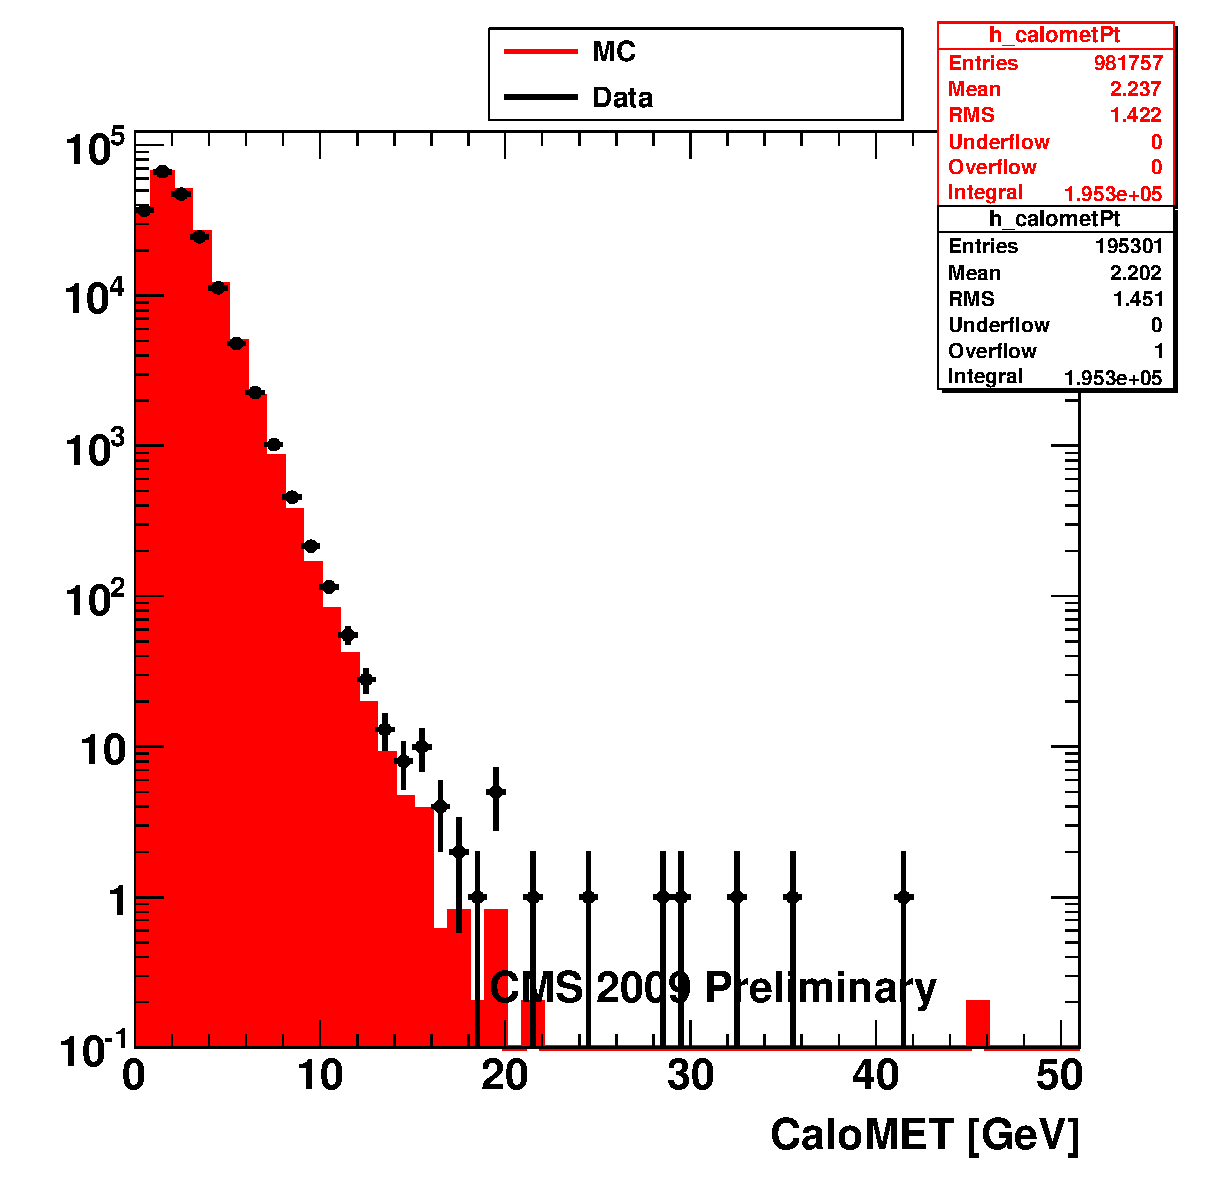
\includegraphics[width=0.40\textwidth]{plots_DataVsMC_MB_900GeV/h_calometPt.eps} &
  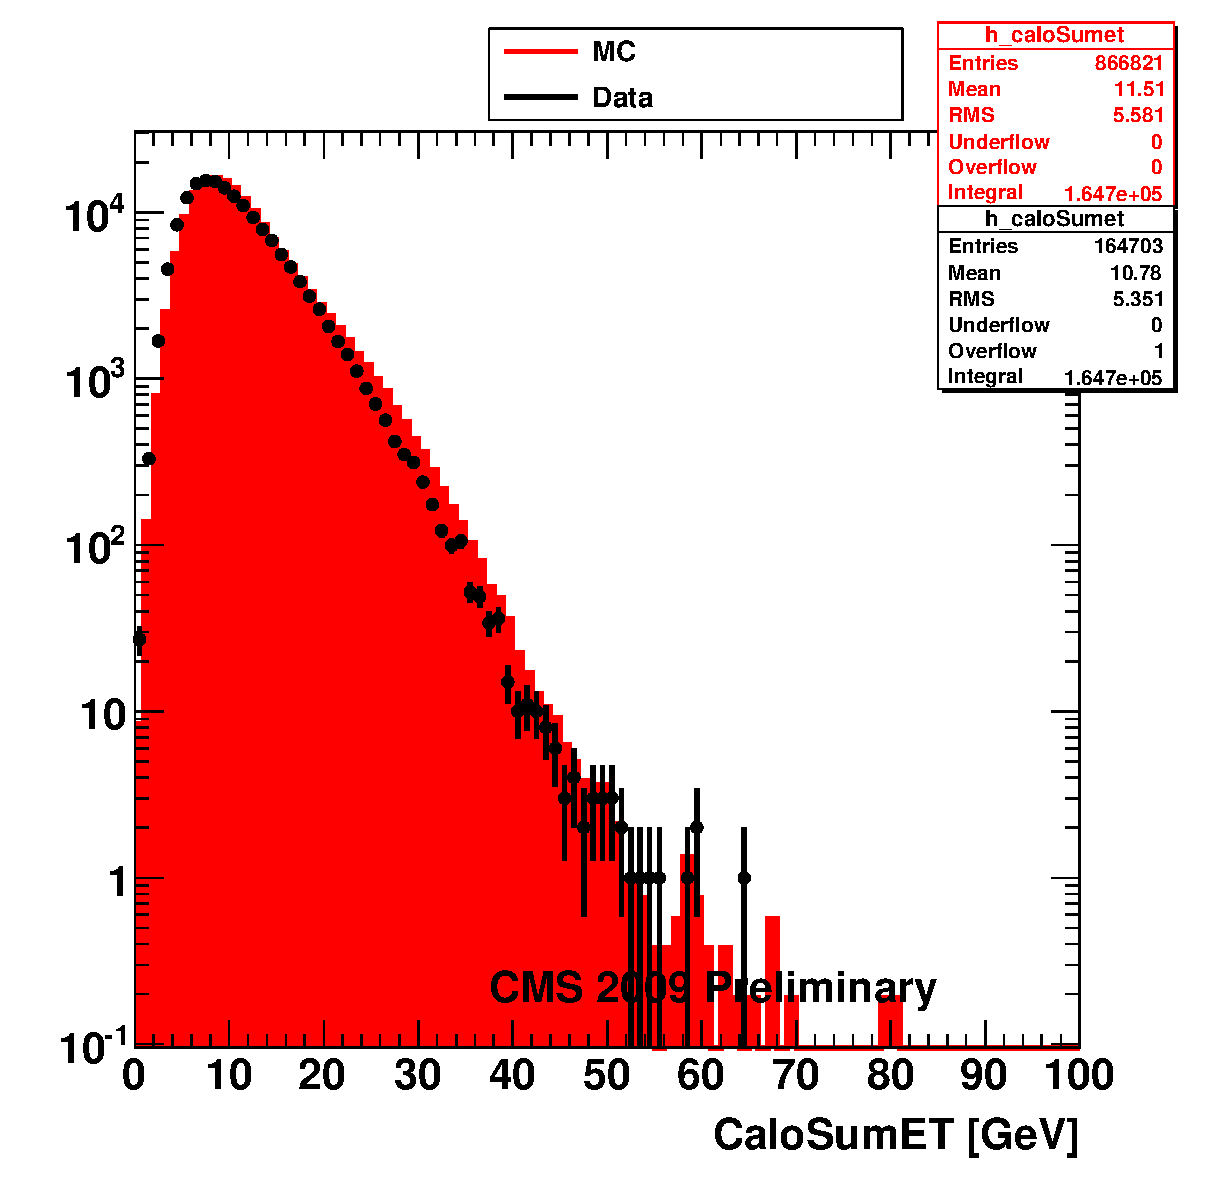
\includegraphics[width=0.40\textwidth]{plots_DataVsMC_MB_900GeV/h_caloSumet.eps} \\
 \end{tabular}
 \caption{$\etmiss$ and SumET distributions in 900 GeV data compared
   with Monte Carlo simulation.
          \label{fig:DataVsMC_MB_900_1}}
\end{figure}

\begin{figure}[h!]
 \centering
 \begin{tabular}{ll}
  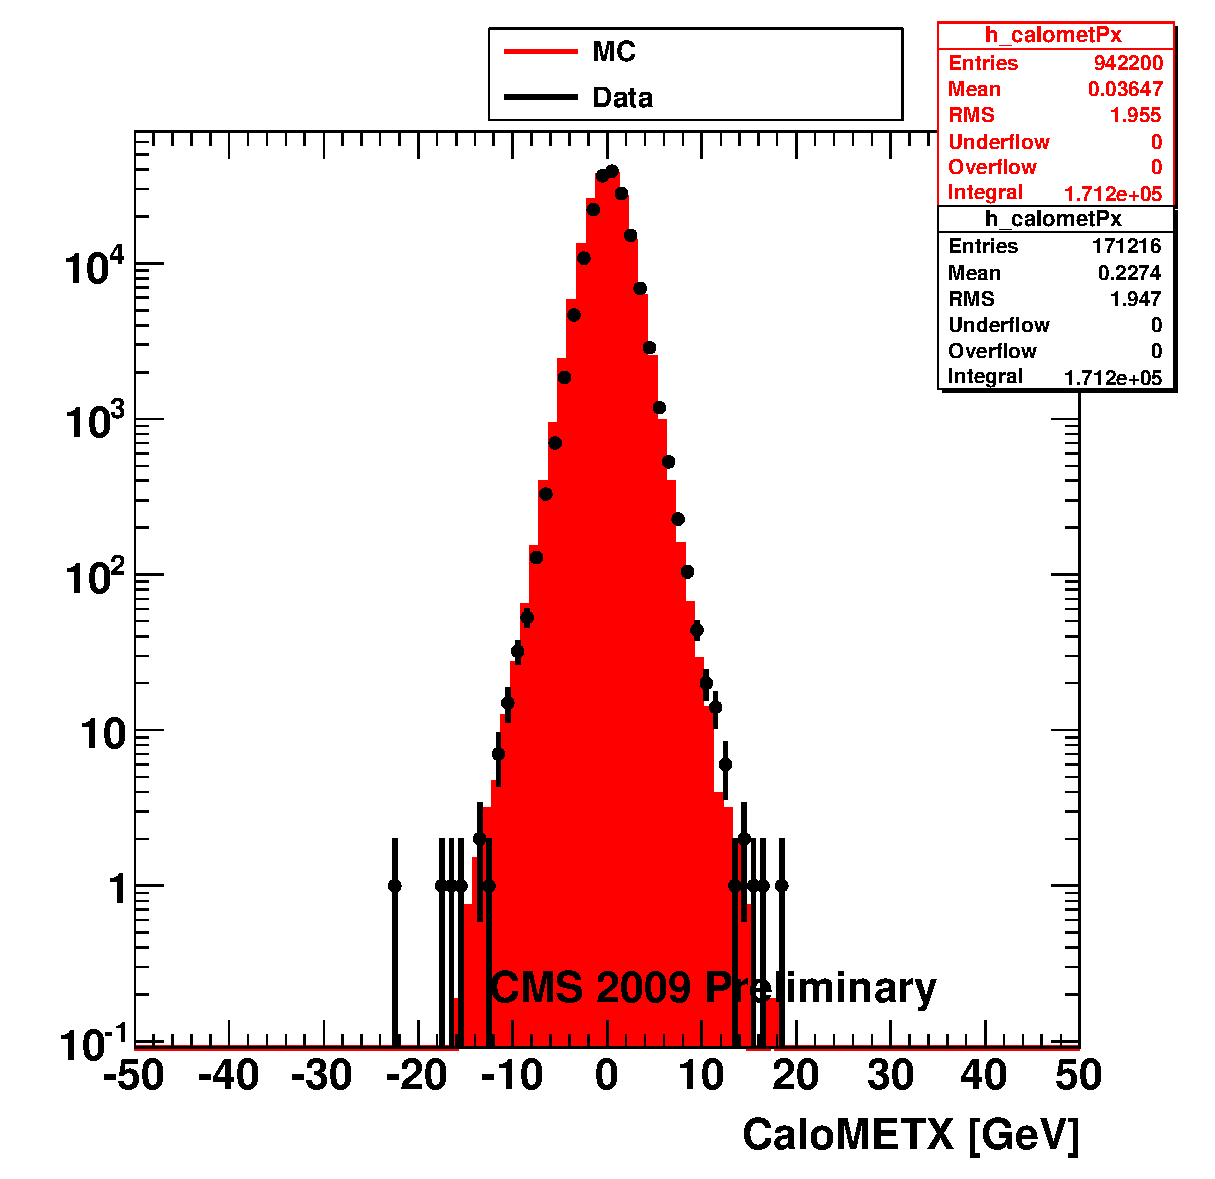
\includegraphics[width=0.40\textwidth]{plots_DataVsMC_MB_900GeV/h_calometPx.eps} &
  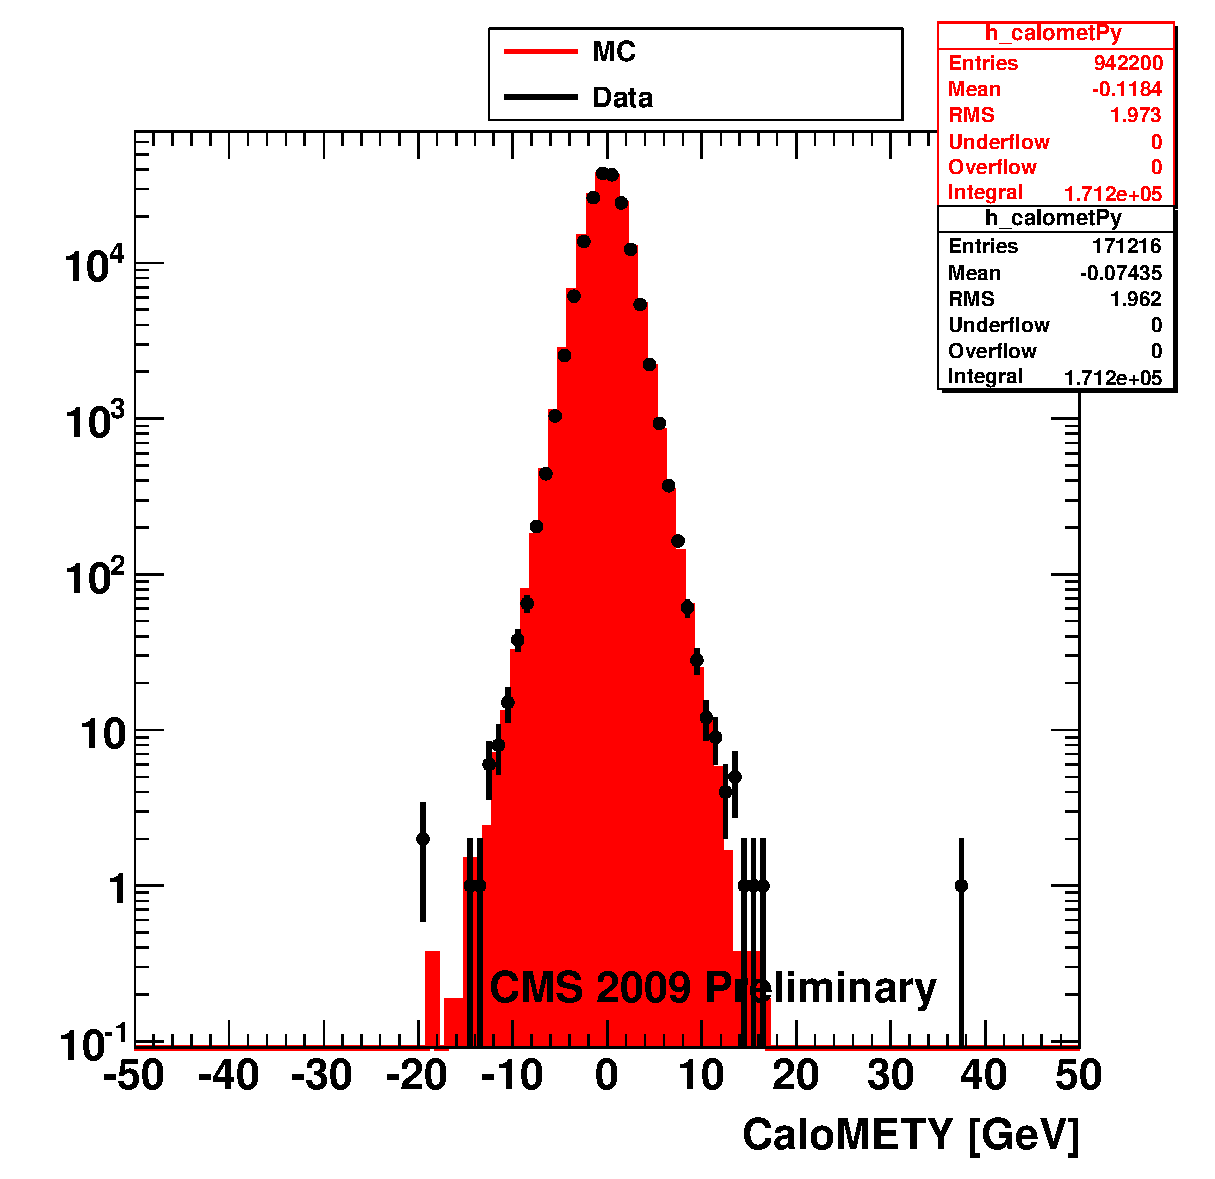
\includegraphics[width=0.40\textwidth]{plots_DataVsMC_MB_900GeV/h_calometPy.eps} \\
 \end{tabular}
 \caption{$\exmiss$ and $\eymiss$ distributions in 900 GeV data compared
   with Monte Carlo simulation.
          \label{fig:DataVsMC_MB_900_2}}
\end{figure}

\begin{figure}[h!]
 \centering
 \begin{tabular}{ll}
  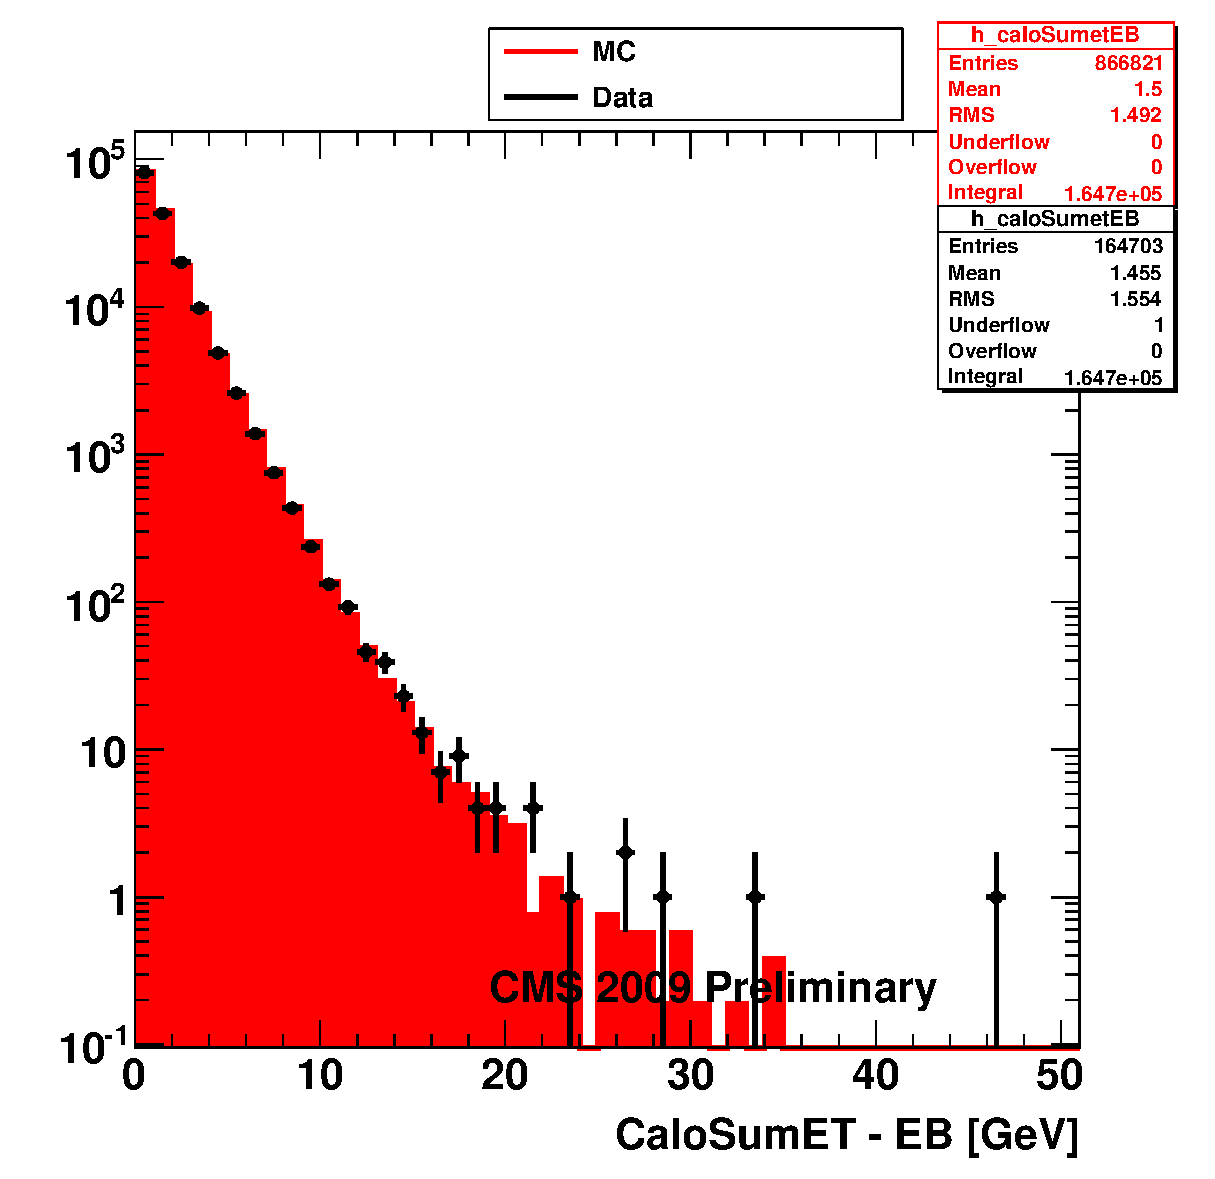
\includegraphics[width=0.40\textwidth]{plots_DataVsMC_MB_900GeV/h_caloSumetEB.eps} &
  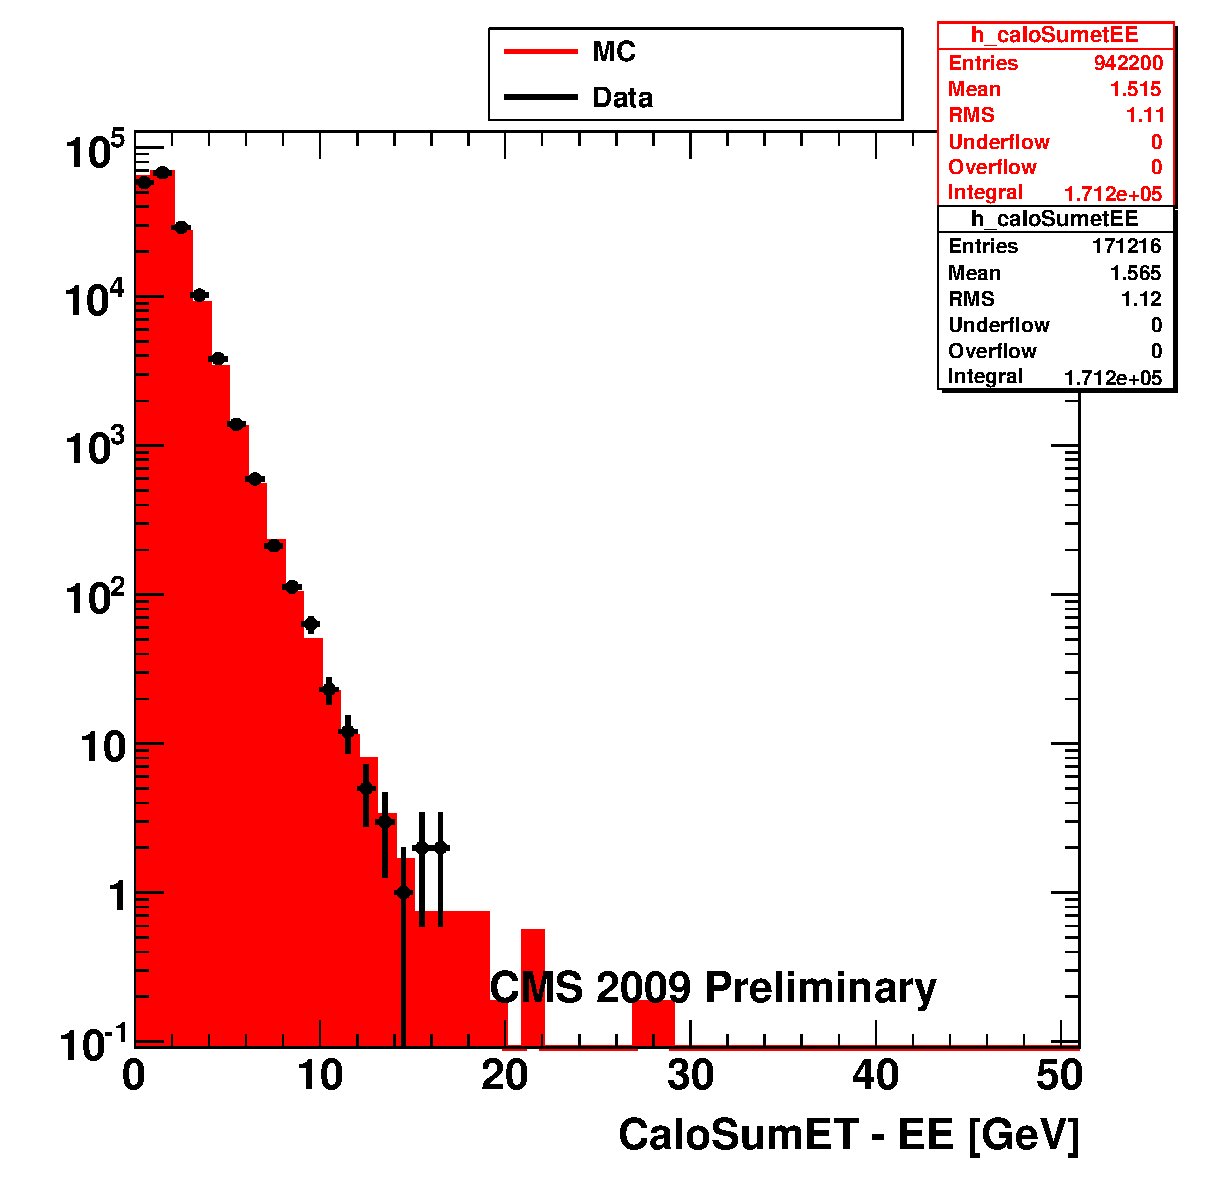
\includegraphics[width=0.40\textwidth]{plots_DataVsMC_MB_900GeV/h_caloSumetEE.eps} \\
 \end{tabular}
 \caption{SumET in ECAL barrel and endcap in 900 GeV data compared
   with Monte Carlo simulation.
          \label{fig:DataVsMC_MB_900_4}}
\end{figure}

\begin{figure}[h!]
 \centering
 \begin{tabular}{ll}
  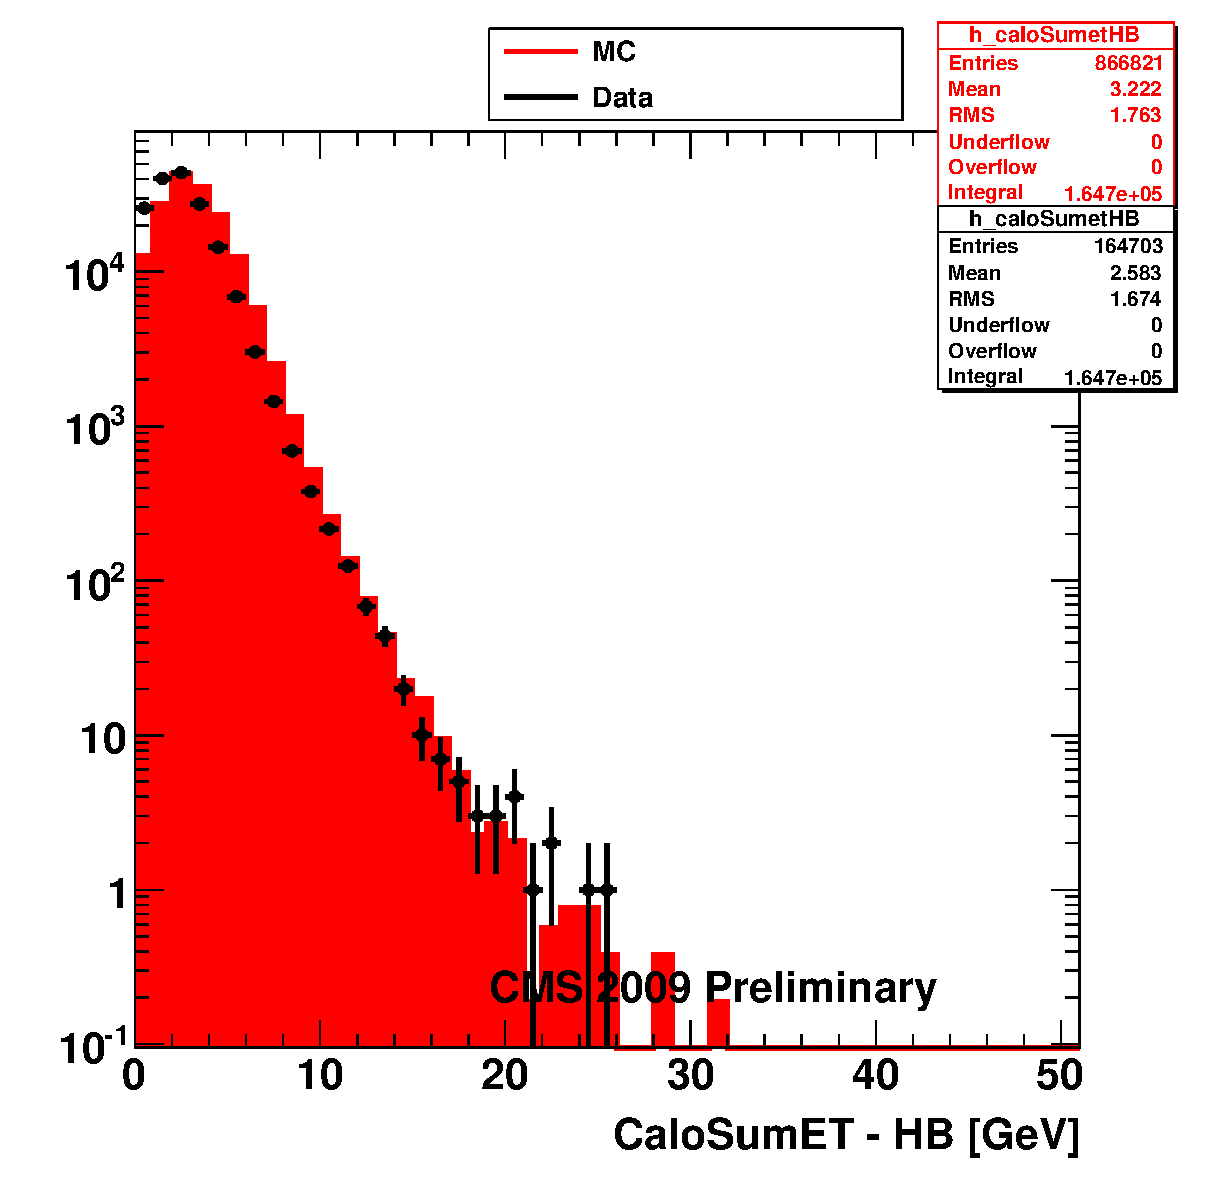
\includegraphics[width=0.40\textwidth]{plots_DataVsMC_MB_900GeV/h_caloSumetHB.eps} &
  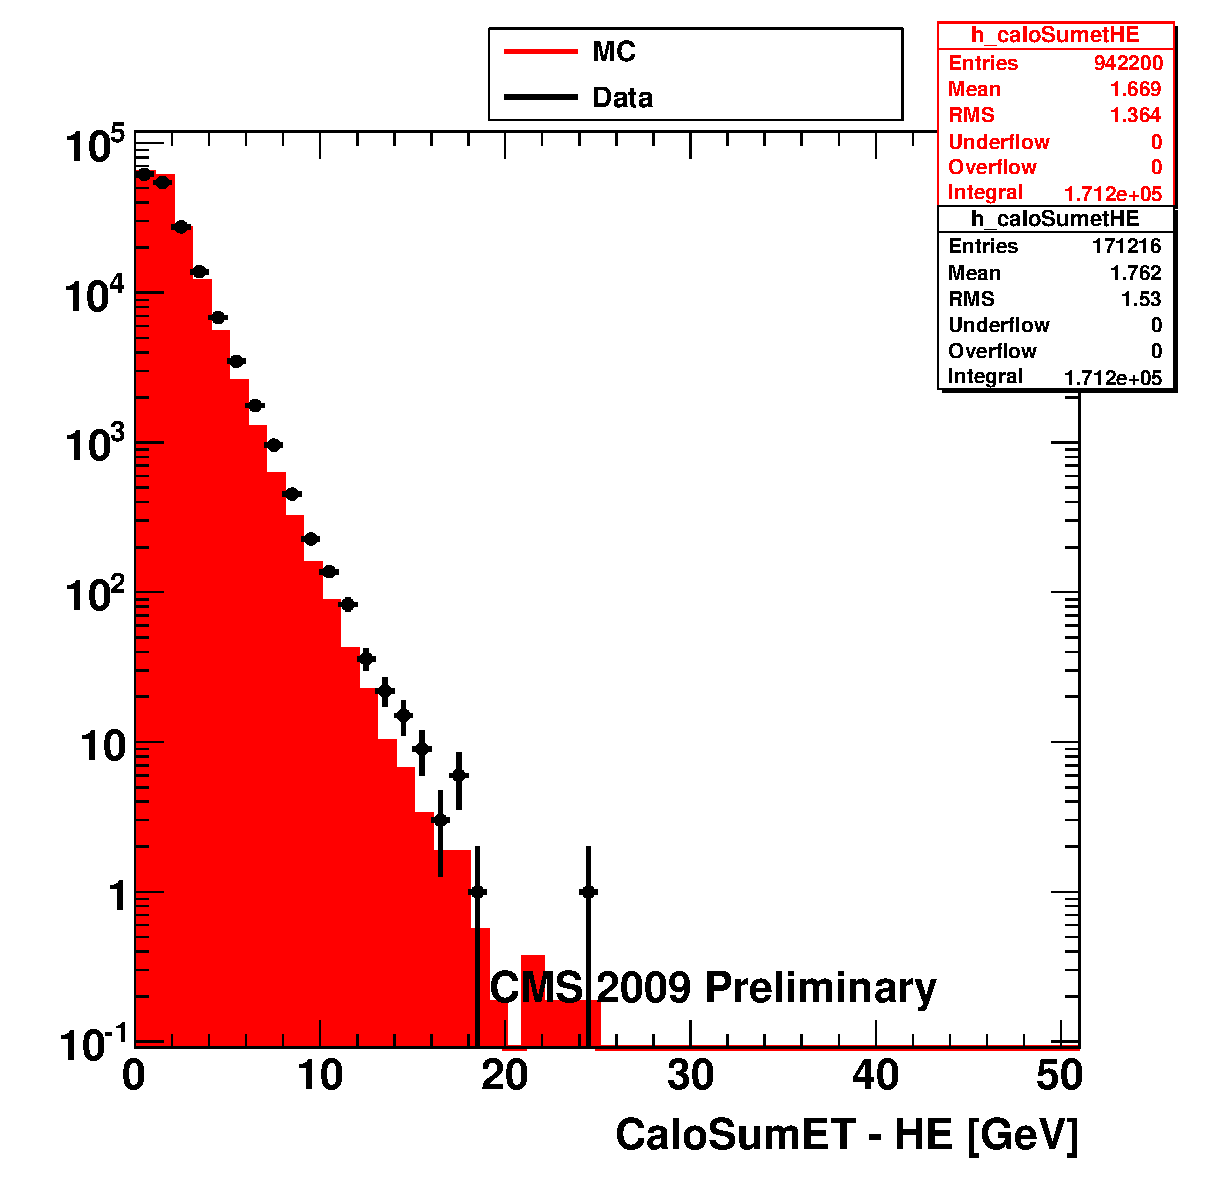
\includegraphics[width=0.40\textwidth]{plots_DataVsMC_MB_900GeV/h_caloSumetHE.eps} \\
 \end{tabular}
 \caption{SumET in HCAL barrel and endcap in 900 GeV data compared
   with Monte Carlo simulation.
          \label{fig:DataVsMC_MB_900_5}}
\end{figure}

\begin{figure}[h!]
 \centering
 \begin{tabular}{ll}
  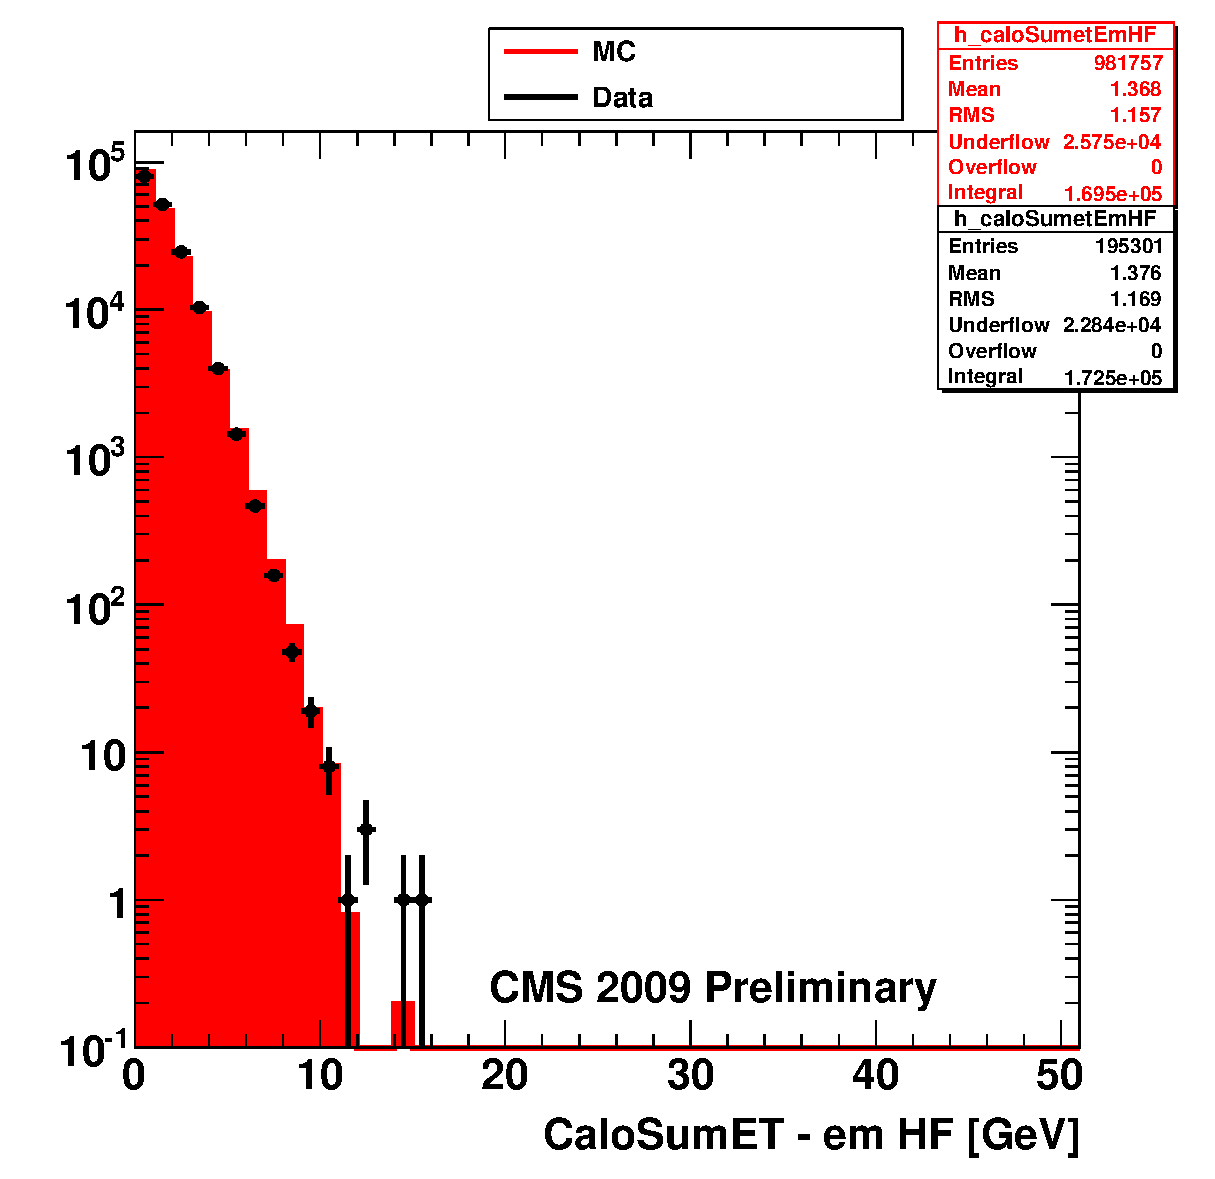
\includegraphics[width=0.40\textwidth]{plots_DataVsMC_MB_900GeV/h_caloSumetEmHF.eps} &
  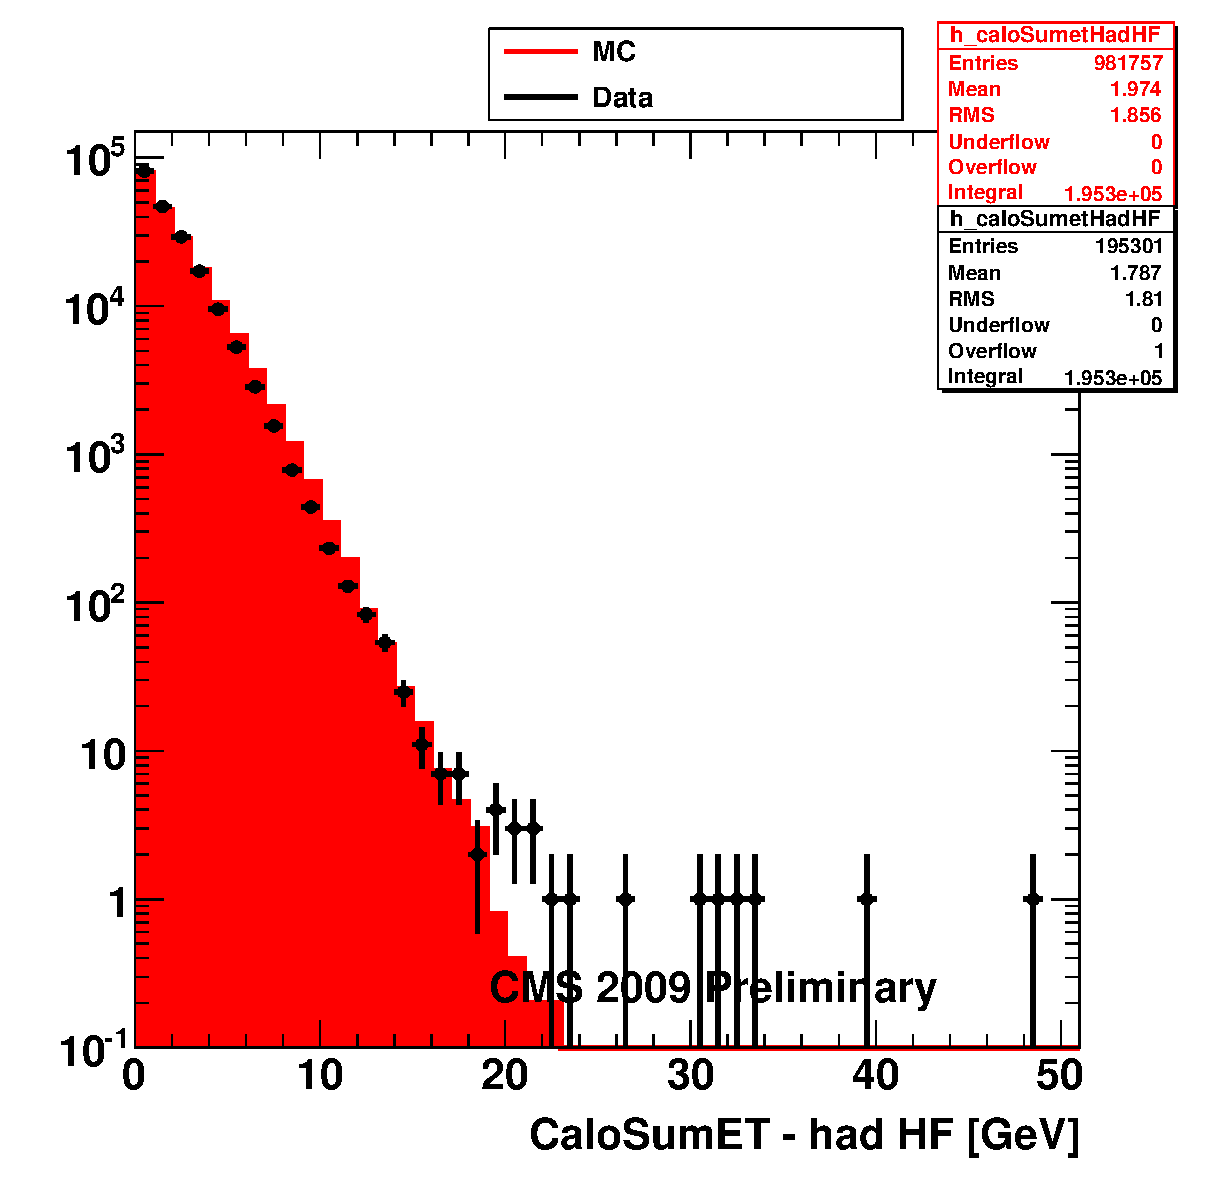
\includegraphics[width=0.40\textwidth]{plots_DataVsMC_MB_900GeV/h_caloSumetHadHF.eps} \\
 \end{tabular}
 \caption{SumET in HF in electromagnetic and hadronic parts in 900 GeV data compared
   with Monte Carlo simulation.
          \label{fig:DataVsMC_MB_900_6}}
\end{figure}

Some of the features of the high $\etmiss$ events are listed below:
\begin{itemize}
\item Run 124024, ls 52, event 19351796: $\etmiss=41.04$~GeV. looks
like an HF PMT hit.
\item Run 124027, ls 33, event 11536636: $\etmiss=32.38$~GeV, likely coming from HPD noise.
\item Run 124020, ls 57, event: 20853863: $\etmiss=24.7$~GeV, looks like
noise in HB, no energy deposit in ECAL at all in the event.
\item Run 124027, ls 35, event 12262783: $\etmiss=21.2045$~GeV, looks like a
HF PMT hit.
\item Run 124030, ls 14, event 4893420: $\etmiss=19.987$~GeV, looks like a 4
jet event which are back-to-back and one is undermeasured.
\item Run 124030, ls 8, event 2665873:  $\etmiss=19.735$~GeV, looks like an HF
PMT hit.
\item Run 124023, ls 46, event 5522301: $\etmiss=19.5925$~GeV, looks like a noise in HB.
\item Run 124024, ls 78, event 28980731: $\etmiss=19.533$~GeV, not clear,
looks like a real energy deposit in a few neihboring HF towers.
\item Run 124024, ls 35, event 13000542: $\etmiss=19.1684$~GeV, an isolated
ECAL tower, but there are tracks pointing to it.
\item Run 124020, ls 35, event 12386199: $\etmiss=17.3609$~GeV,
  undermeasured energy, many soft deposits here and there.
\item Run 124023, ls 50, event 6957103: $\etmiss=16.9166$~GeV, seems to be a
noise event in HB.
\item Run 124020, ls 16, event 5343881: $\etmiss=16.6777$~GeV, looks like an
ECAL spike, but also track pointing to it.
\item Run 124024, ls 80, event 29768956: $\etmiss=16.3216$~GeV, looks like HF
PMT hit.
\item Run 124023, ls: 65, event 12665379: $\etmiss=16.2541$~GeV, noisy tower
in HB
\item Run 124022, ls 122, event: 26573093: $\etmiss=16.0949$~GeV, not clear
\item Run 124023, ls 65, event 12466348: $\etmiss=15.9701$~GeV, HF PMT hit
\item Run 124025, ls 7, event 2194922: $\etmiss=15.946$~GeV, may be HF PMT hit
\item Run 124027, ls 26, event 8792680: $\etmiss=15.9426$~GeV, activity in HB,
not clear
\item Run 124022, ls 117, event 24629137: $\etmiss=15.5451$~GeV, activity in
EB/HB, not clear
\item Run 124023, ls 50, event 7040081:$\etmiss=15.5213$~GeV, a few neihboring
towers in HF, does not look like a PMT hit.
\item Run 123818, ls 3, event: 909463: $\etmiss=15.3908$~GeV, possibly HF PMT
hit, not fully clear.
\item Run 124023, ls 40, event 3015033: $\etmiss=15.3819$~GeV, maybe HF PMT
hit
\item Run 124024, ls 21,  event 7735977: $\etmiss=15.372$~GeV, not clear, some
activity in HB only
\item Run 124022, ls 133, event 30695922: $\etmiss=15.1507$~GeV, not clear, a
tower in HB with a track pointing to it.
\item Run 124022, ls 130, event 29704007: $\etmiss=15.0855$~GeV, not clear,
maybe HB noise.
\end{itemize}

\begin{figure}[h!]
  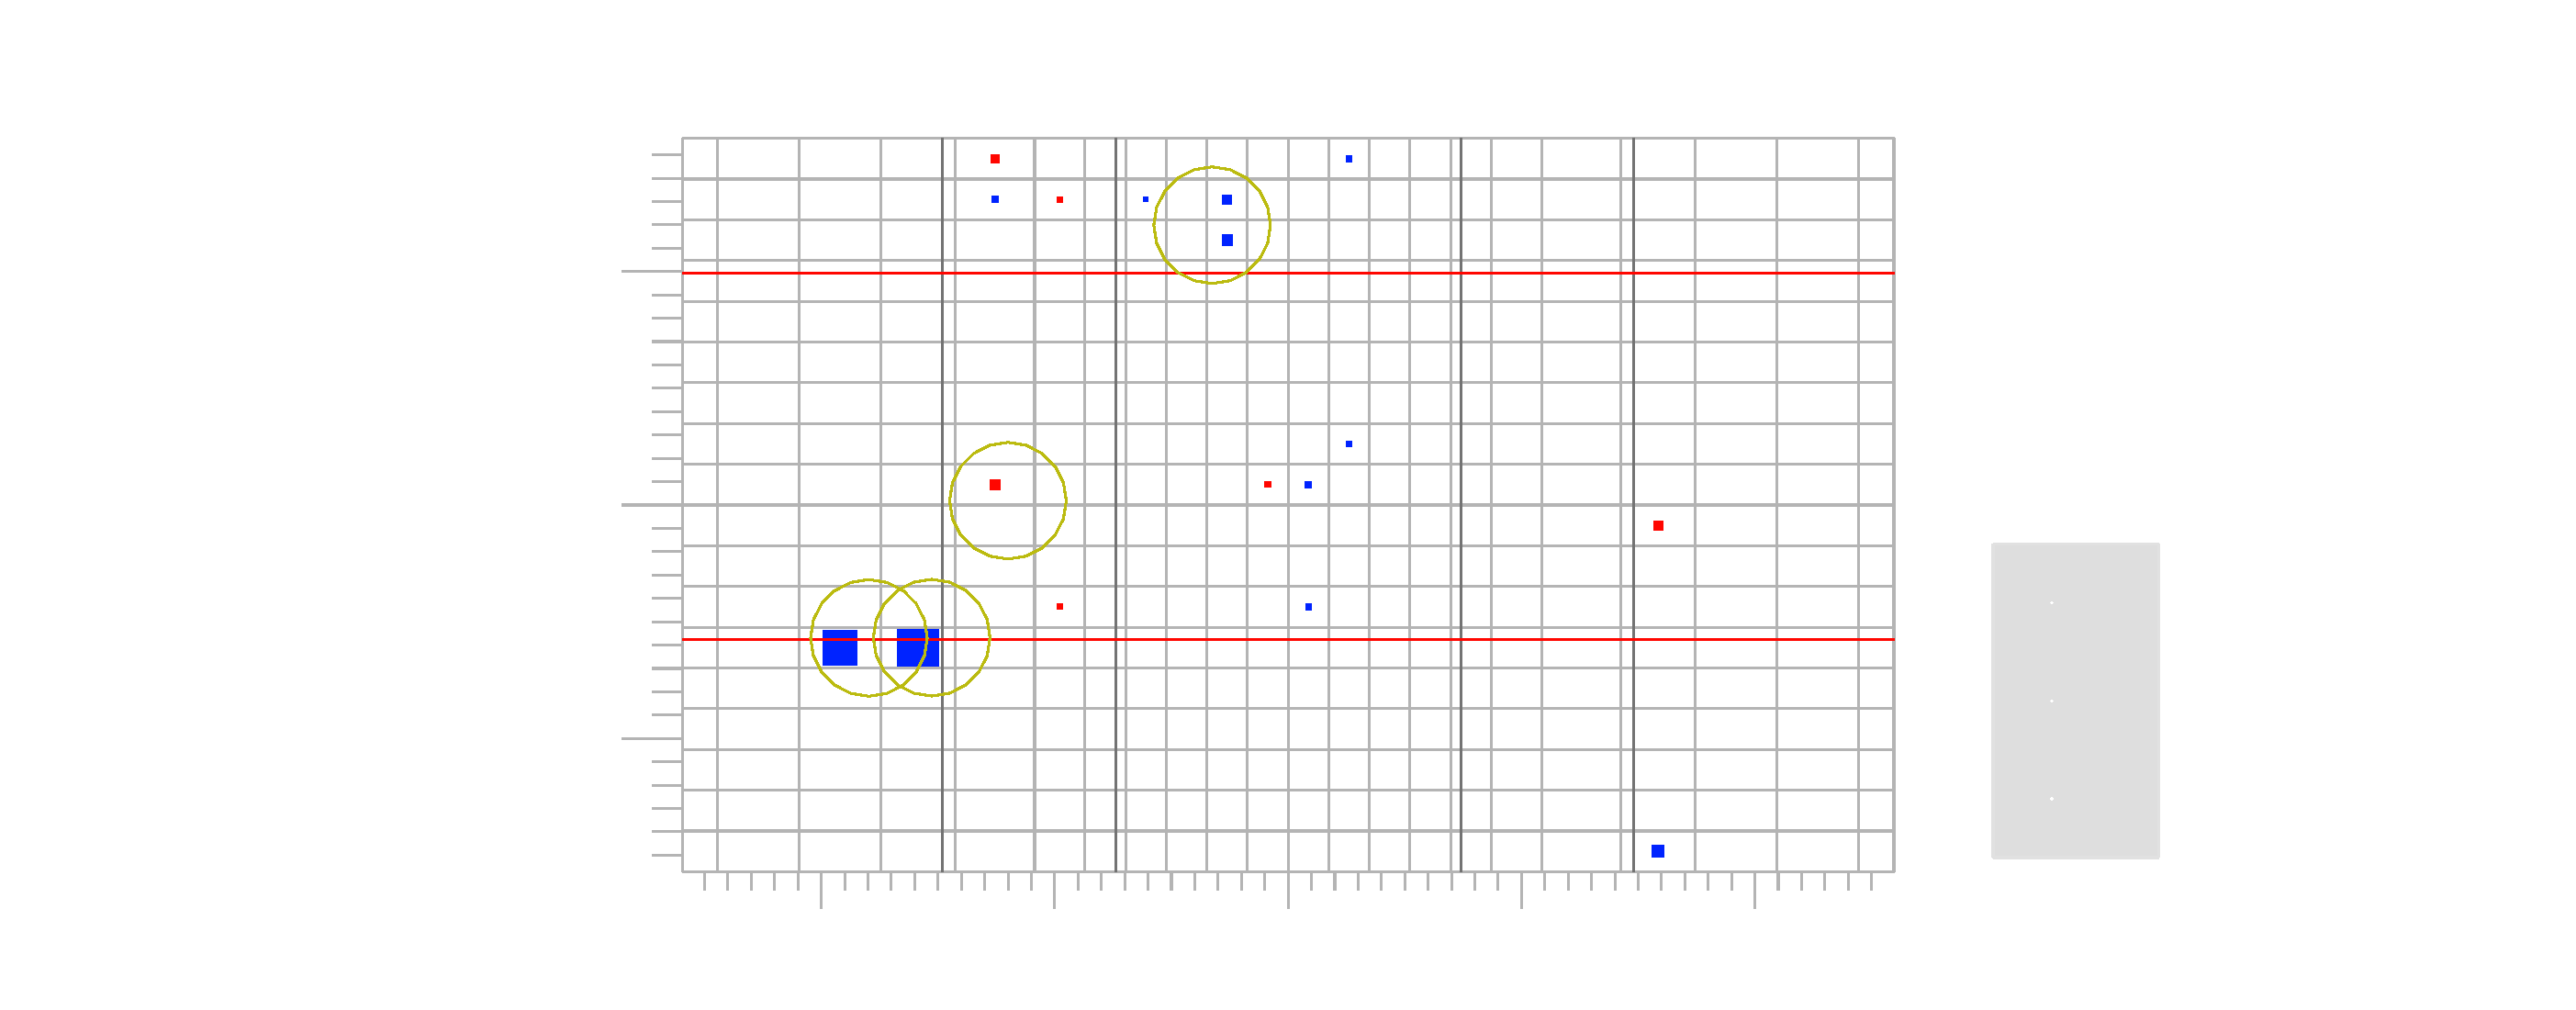
\includegraphics[width=12cm]{plots_DataVsMC_MB_900GeV/124024_19351796_MET41GeV.eps}
  \caption{Lego plot of the highest $\etmiss=41.04$~GeV event (Run 124024, ls 52, event 19351796). It appears
    that the $\etmiss$ is caused by an HF PMT hit.
    \label{fig:DataVsMC_MB_900_evd1}}
\end{figure}

\begin{figure}[h!]
  \includegraphics[width=12cm]{plots_DataVsMC_MB_900GeV/124027_11536636_HPD.eps}
  \caption{Lego plot of the $\etmiss=32.38$~GeV event (Run 124027, ls 33, event 11536636). The multiplicity
    of HCAL towers suggests that this event is cause by HPD discharge.
    \label{fig:DataVsMC_MB_900_evd2}}
\end{figure}

\begin{figure}[h!]
  \includegraphics[width=12cm]{plots_DataVsMC_MB_900GeV/124030_4893420_4jet.eps}
  \caption{The $\etmiss=19.987$~GeV event (Run 124030, ls
    14, event 4893420). This event seems to contain 4 jets, one of which
    is severly undermeasured causing the $\etmiss$.
    \label{fig:DataVsMC_MB_900_evd3}}
\end{figure}


\clearpage

\subsection{$\etmiss$ resolution}

For events with no $\etmiss$ from physics sources, the $\etmiss$ resolution can be most generally parameterized
according to the following expression (CMS AN-2007/041):
\begin{equation}
  \sigma\left(\etmiss\right)=A \oplus B\sqrt{\sum E_\text{T}-D} \oplus C\left(\sum E_\text{T}-D\right),
  \label{eq:MET_sigma}
\end{equation}
where $A$ is the noise term, $B$ is the stohastic term, $C$ is the constant term, and $D$ is the offset term. In such events
$\exmiss$ and $\eymiss$ are expected to follow a Gaussian distribution with the mean of zero and the standard deviation
of $\sigma$. It can also be shown that $\sigma\left(\etmiss\right)$ is proportional to this $\sigma$. Therefore,
by looking at $\sigma\left(\exmiss\right)$ and $\sigma\left(\eymiss\right)$ as a function of $\sum E_\text{T}$ it is possible to
study the $\etmiss$ resolution and the relative contributions of different resolution terms at different values of $\sum E_\text{T}$.
Figure~\ref{fig:MExySigma_vs_SumET_900} shows the $\sigma\left(\exmiss\right)$ and $\sigma\left(\eymiss\right)$ 
vs. $\sum E_\text{T}$ for 900 GeV data compared with Monte Carlo simulation. $\sigma\left(\exmiss\right)$ and $\sigma\left(\eymiss\right)$
were extracted from a Gaussian fit to $\exmiss$ and $\eymiss$ distributions, respectively, in a region of $\pm 1.5$ RMS around the mean.
Figures~\ref{fig:MExSigma_vs_SumET_900_fit} and \ref{fig:MEySigma_vs_SumET_900_fit} show the fit of $\sigma\left(\exmiss\right)$
 and $\sigma\left(\eymiss\right)$ vs. $\sum E_\text{T}$ to Eq.~\ref{eq:MET_sigma} for data and Monte Carlo at $900$ GeV.
The offset term $D$, which from results presented in Section~\ref{sc:CaloNoise} is expected to be small, had to be fixed to zero in 
order to get a stable fit.

\begin{figure}[h!]
 \centering
 \begin{tabular}{ll}
  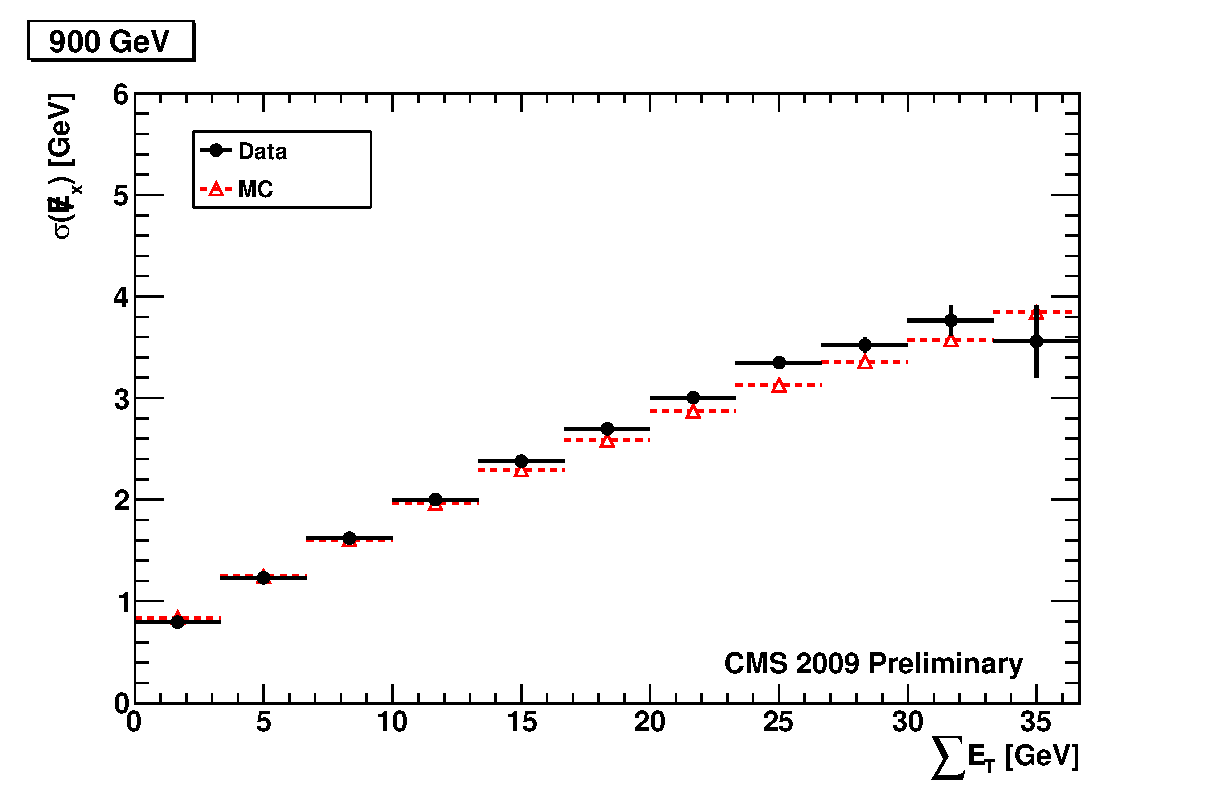
\includegraphics[width=0.5\textwidth]{plots_DataVsMC_MB_900GeV/h_metxsigma_sumet_900.eps} &
  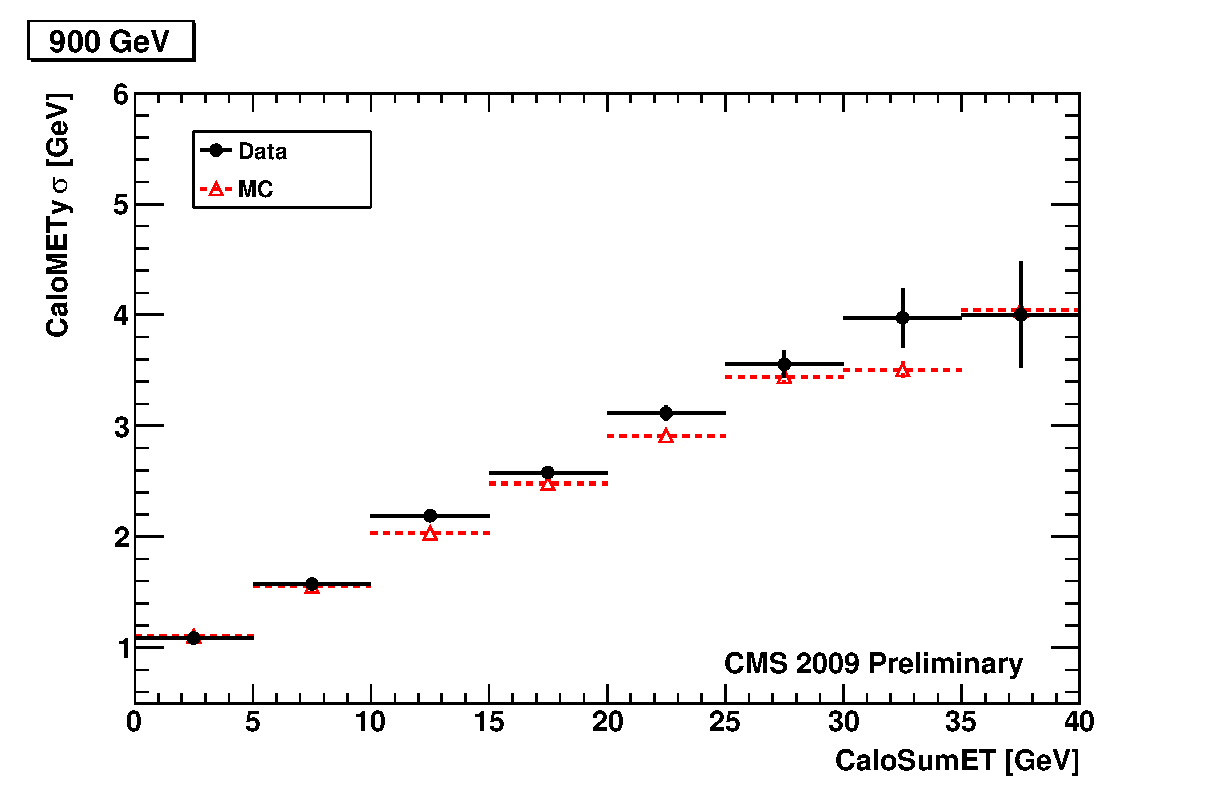
\includegraphics[width=0.5\textwidth]{plots_DataVsMC_MB_900GeV/h_metysigma_sumet_900.eps} \\
 \end{tabular}
 \caption{\small $\sigma\left(\exmiss\right)$ and $\sigma\left(\eymiss\right)$ vs. $\sum E_\text{T}$ for data at $900$ GeV
          compared with Monte Carlo simulation.\label{fig:MExySigma_vs_SumET_900}}
\end{figure}

\begin{figure}[h!]
 \centering
 \begin{tabular}{ll}
  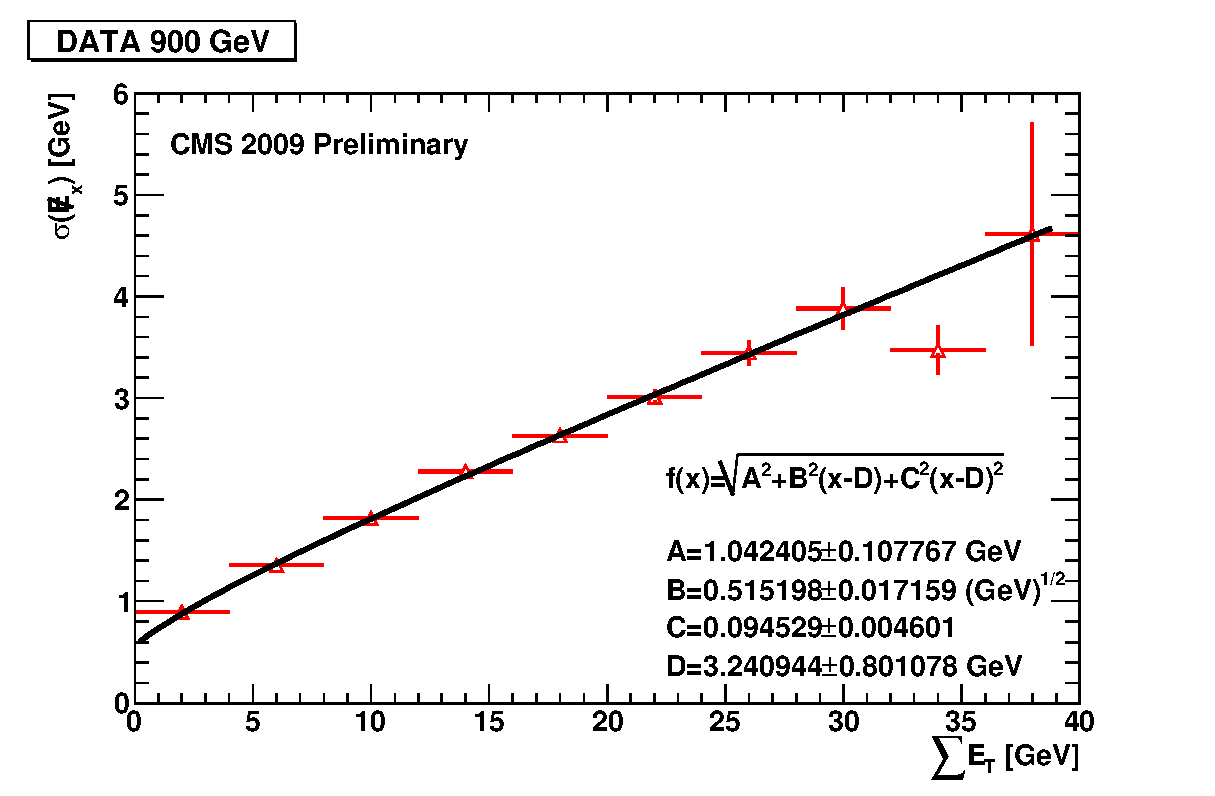
\includegraphics[width=0.5\textwidth]{plots_DataVsMC_MB_900GeV/final_metxsigma_sumet_DATA_900.eps} &
  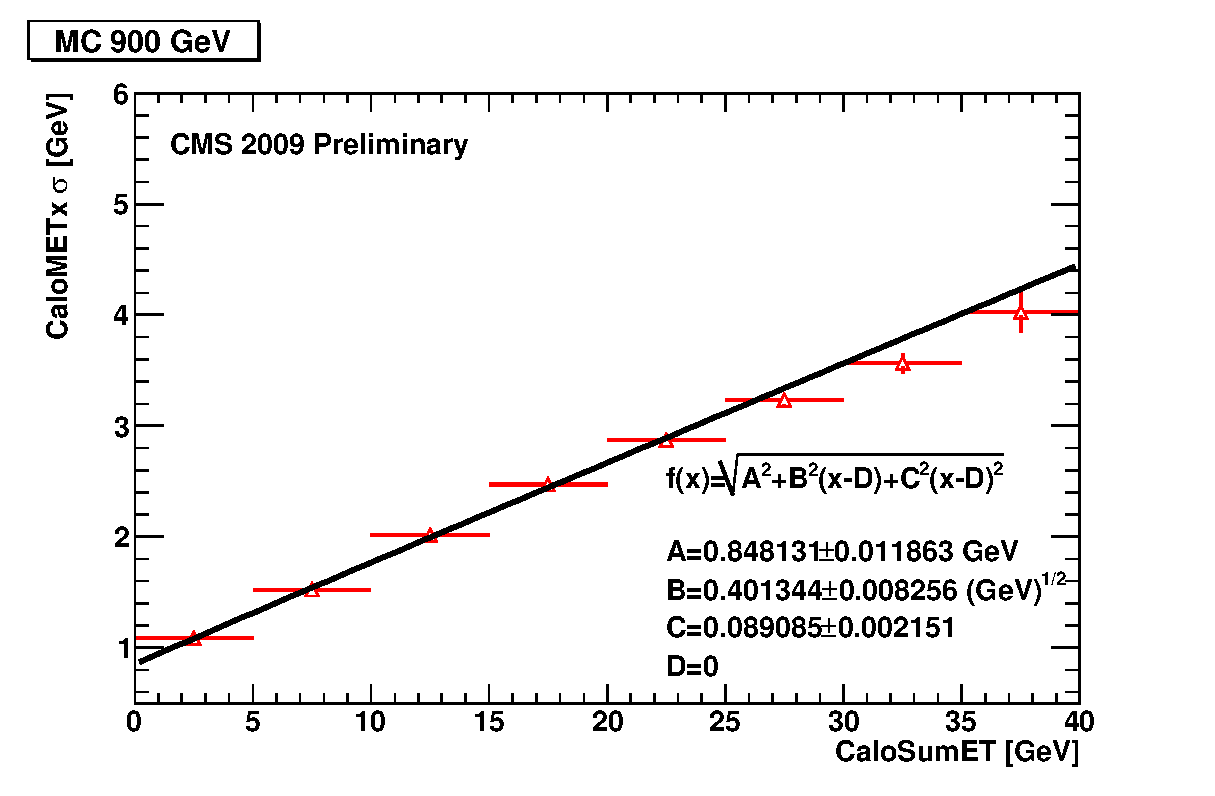
\includegraphics[width=0.5\textwidth]{plots_DataVsMC_MB_900GeV/final_metxsigma_sumet_MC_900.eps} \\
 \end{tabular}
 \caption{\small Fit of the $\sigma\left(\exmiss\right)$ vs. $\sum E_\text{T}$ for data and Monte Carlo at $900$ GeV. Parameter $D$ in the fit was fixed
          to zero.\label{fig:MExSigma_vs_SumET_900_fit}}
\end{figure}

\begin{figure}[h!]
 \centering
 \begin{tabular}{ll}
  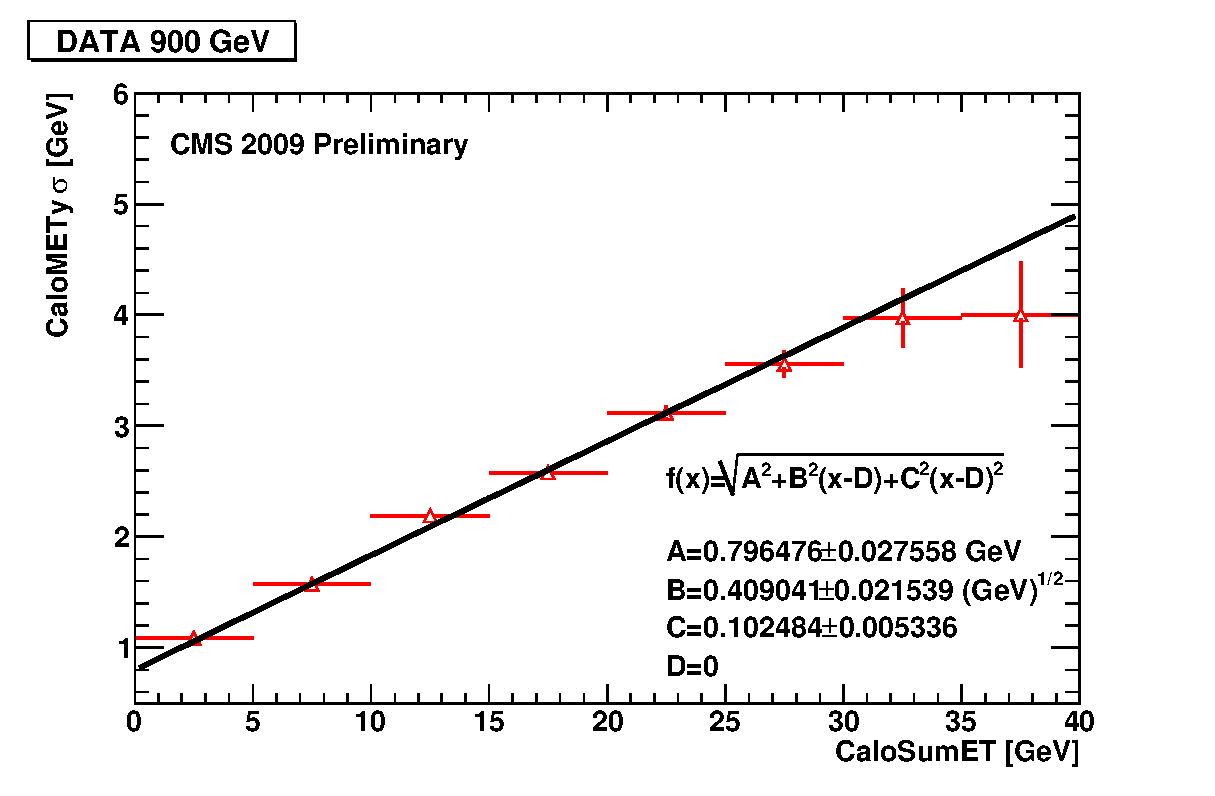
\includegraphics[width=0.5\textwidth]{plots_DataVsMC_MB_900GeV/final_metysigma_sumet_DATA_900.eps} &
  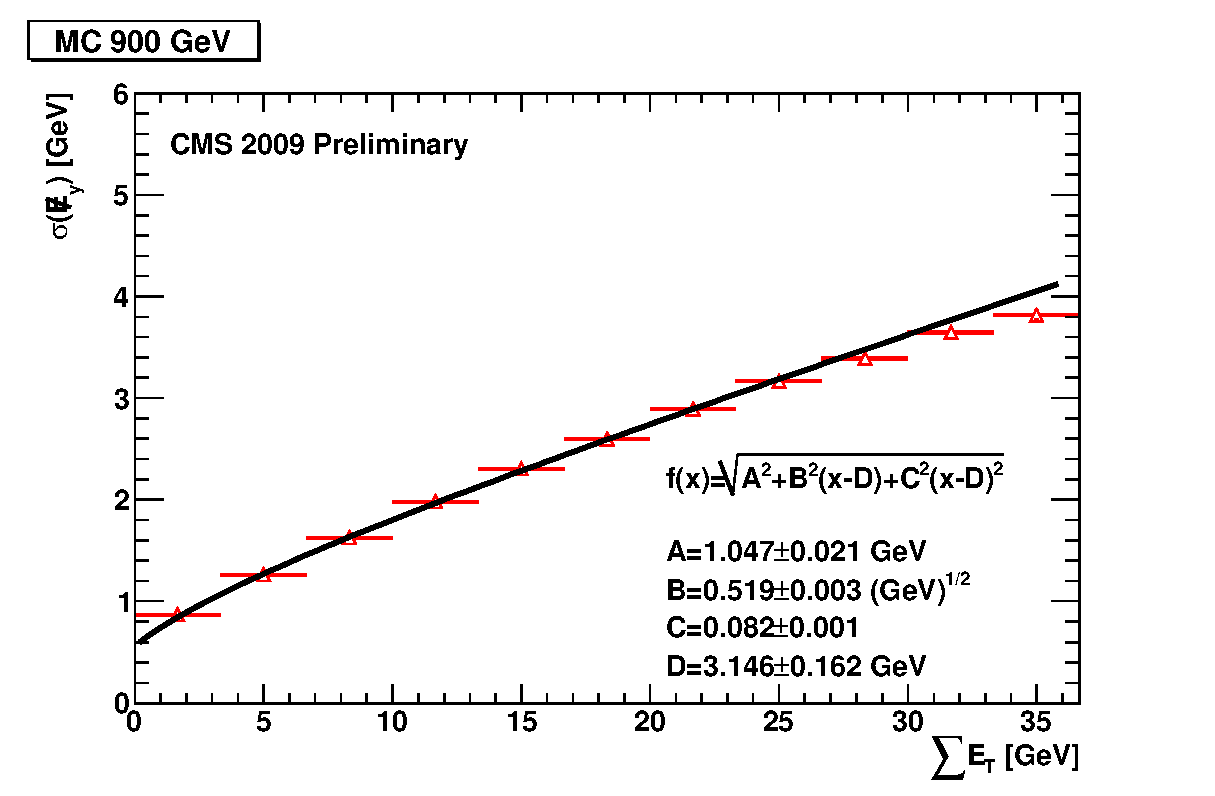
\includegraphics[width=0.5\textwidth]{plots_DataVsMC_MB_900GeV/final_metysigma_sumet_MC_900.eps} \\
 \end{tabular}
 \caption{\small Fit of the $\sigma\left(\eymiss\right)$ vs. $\sum E_\text{T}$ for data and Monte Carlo at $900$ GeV. Parameter $D$ in the fit was fixed
          to zero.\label{fig:MEySigma_vs_SumET_900_fit}}
\end{figure}


\clearpage

\subsection{$\etmiss$ and SumET dependence on $\eta$}

\begin{figure}[h!]
 \centering
 \begin{tabular}{ll}
  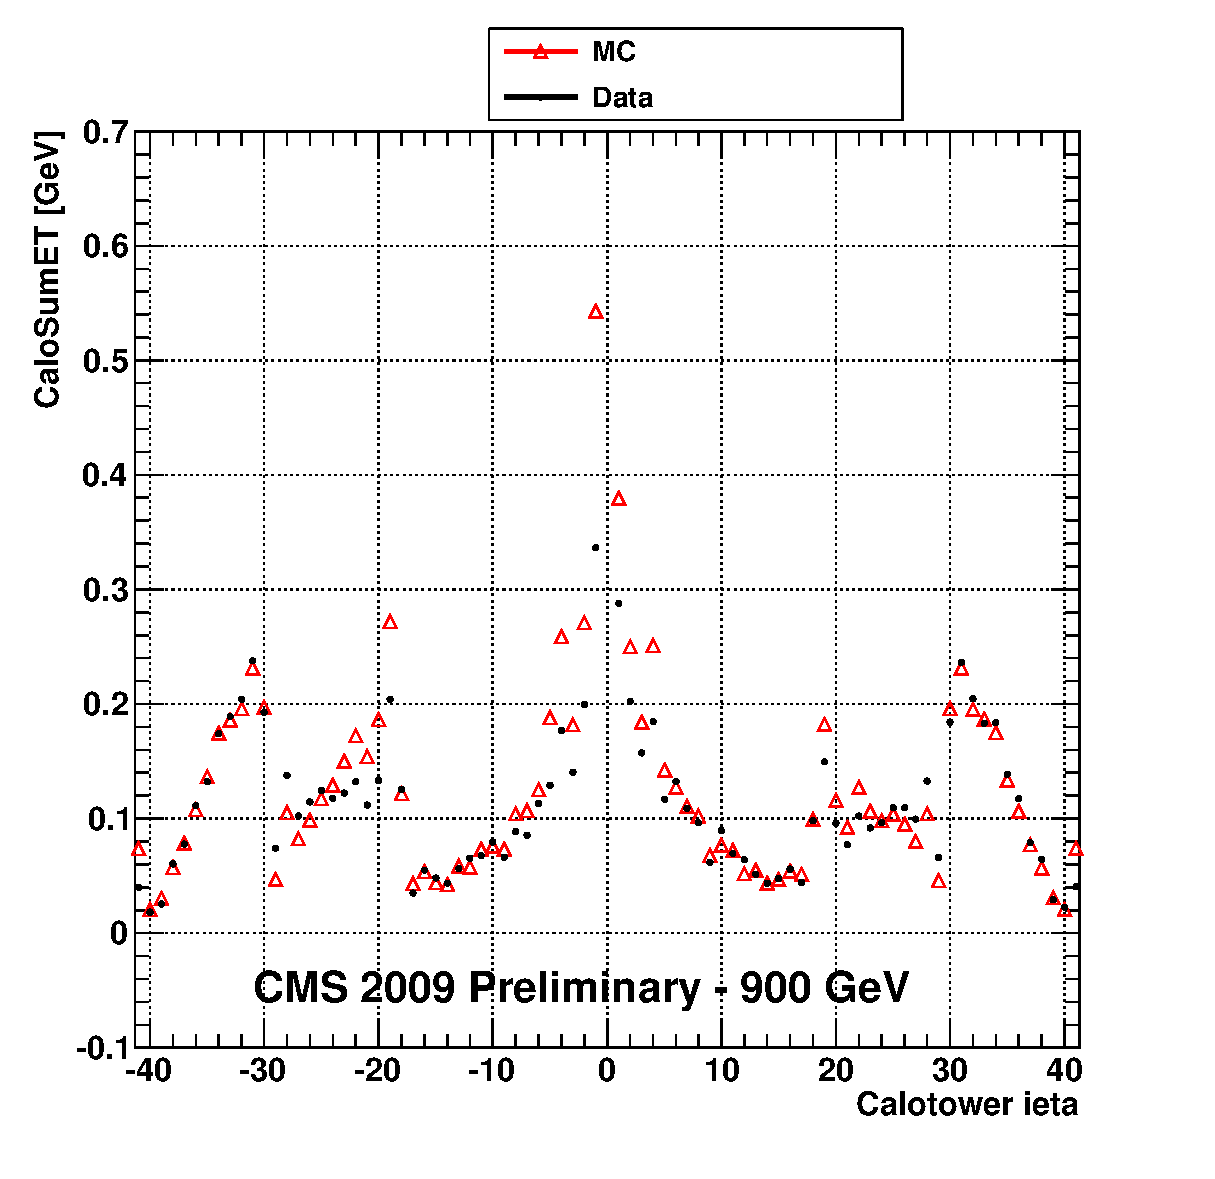
\includegraphics[width=0.5\textwidth]{plots_DataVsMC_MB_900GeV/g_caloSumetMean_vs_ieta_900.eps} &
  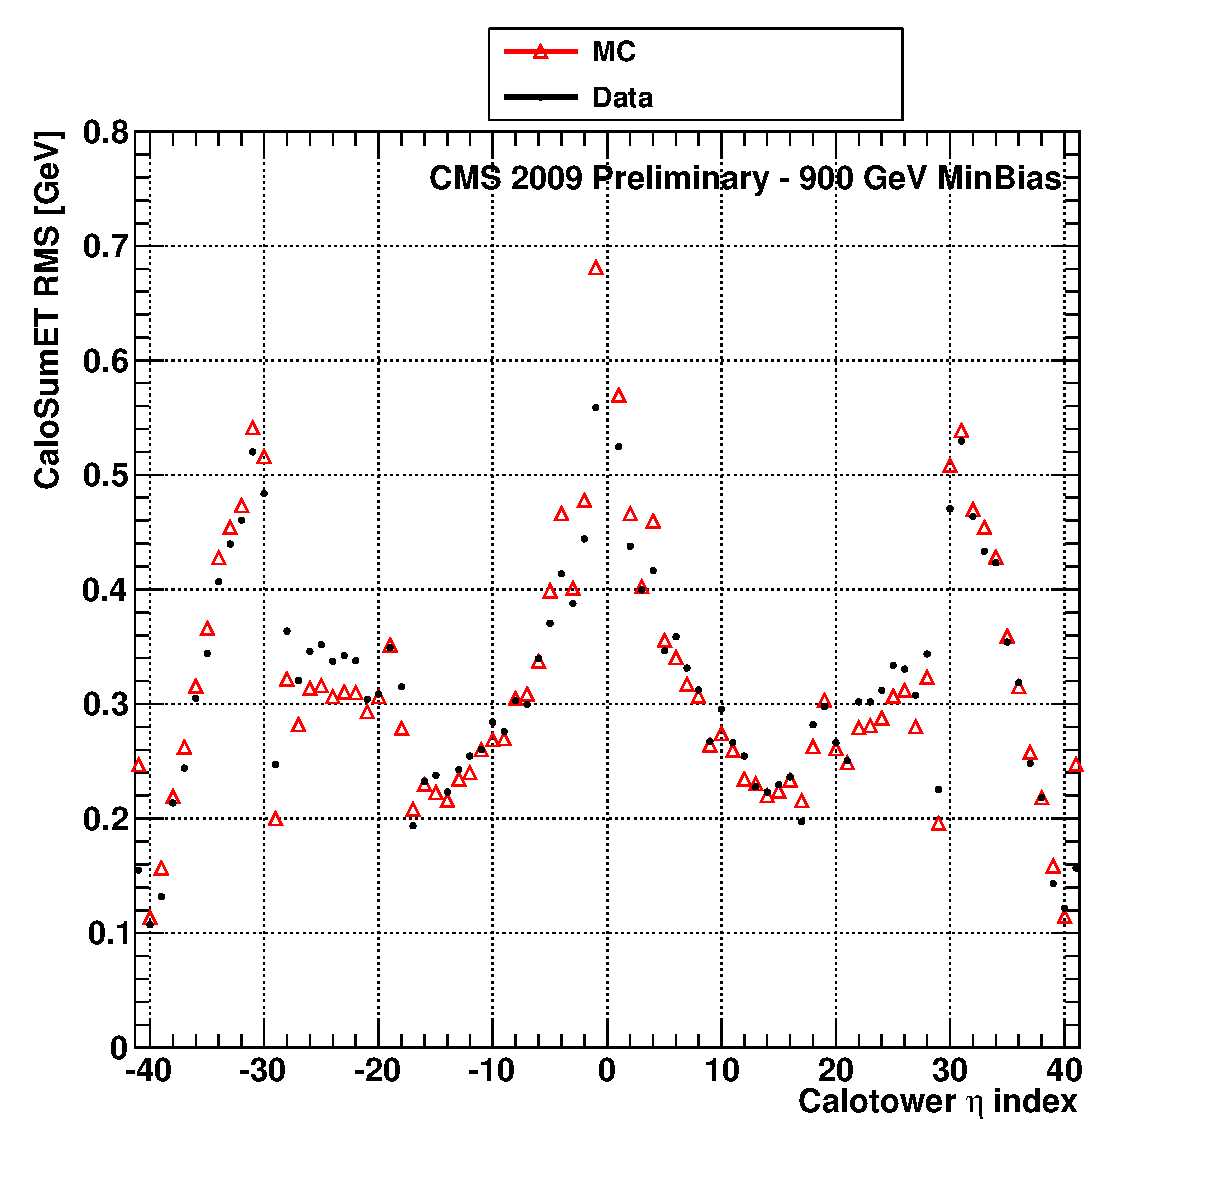
\includegraphics[width=0.5\textwidth]{plots_DataVsMC_MB_900GeV/g_caloSumetRMS_vs_ieta_900.eps} \\
 \end{tabular}
 \caption{\small Comparison of the SumET Mean vs. i$\eta$ of calotowers and SumET RMS vs. i$\eta$ of calotowers between 
          Monte Carlo and data at $900$ GeV.\label{fig:SumET_MeanRMS_vs_ieta_900}}
\end{figure}

\begin{figure}[h!]
 \centering
 \begin{tabular}{ll}
  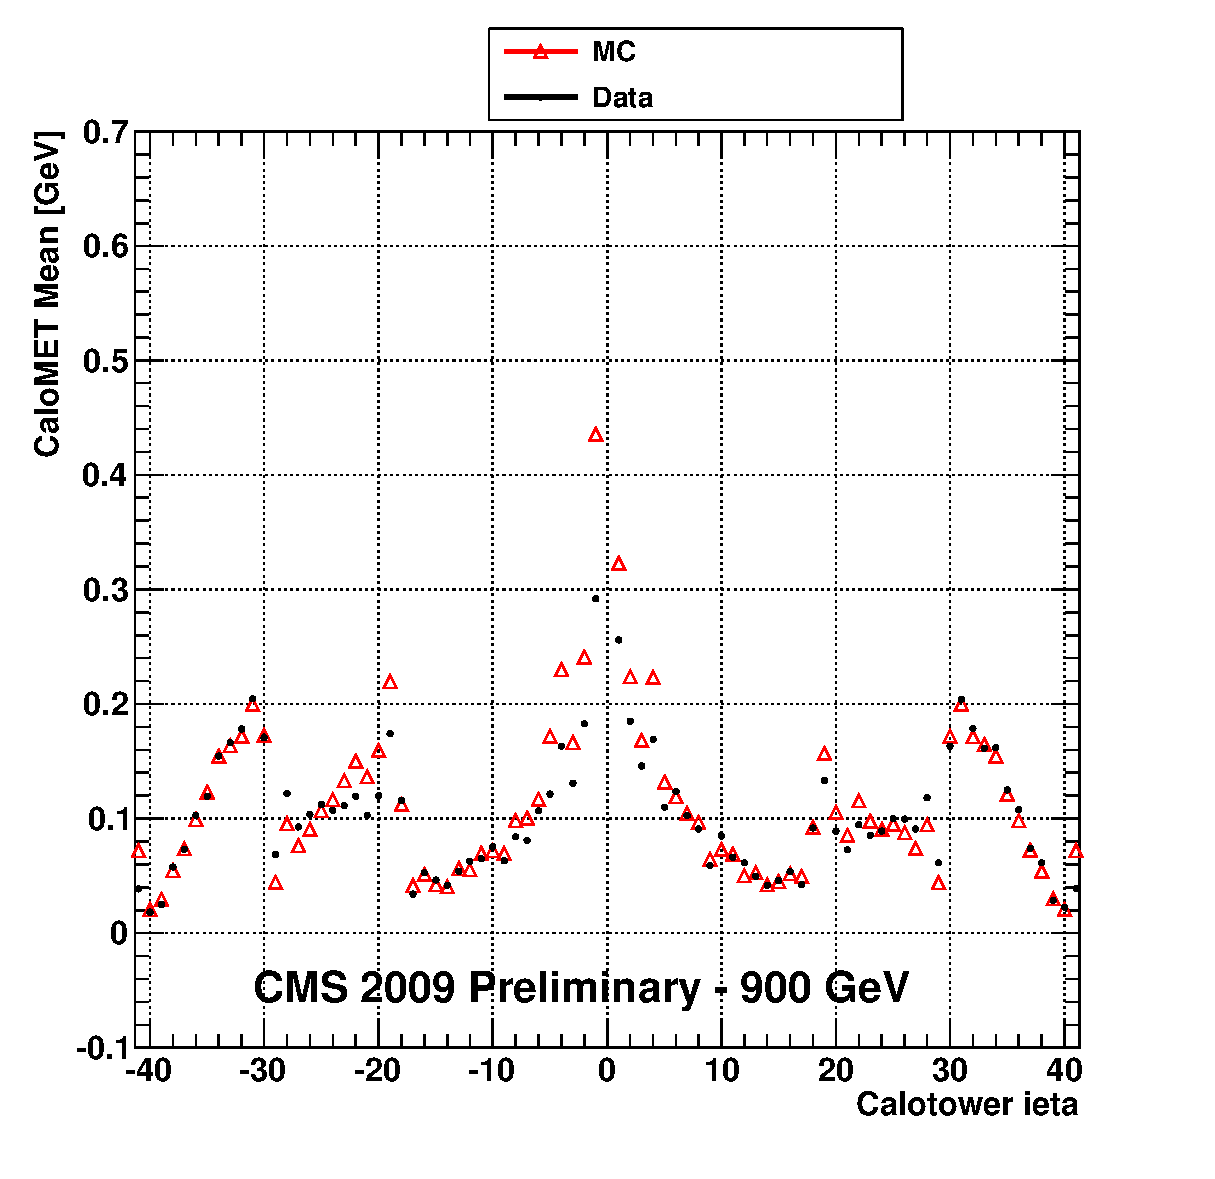
\includegraphics[width=0.5\textwidth]{plots_DataVsMC_MB_900GeV/g_calometPtMean_vs_ieta_900.eps} &
  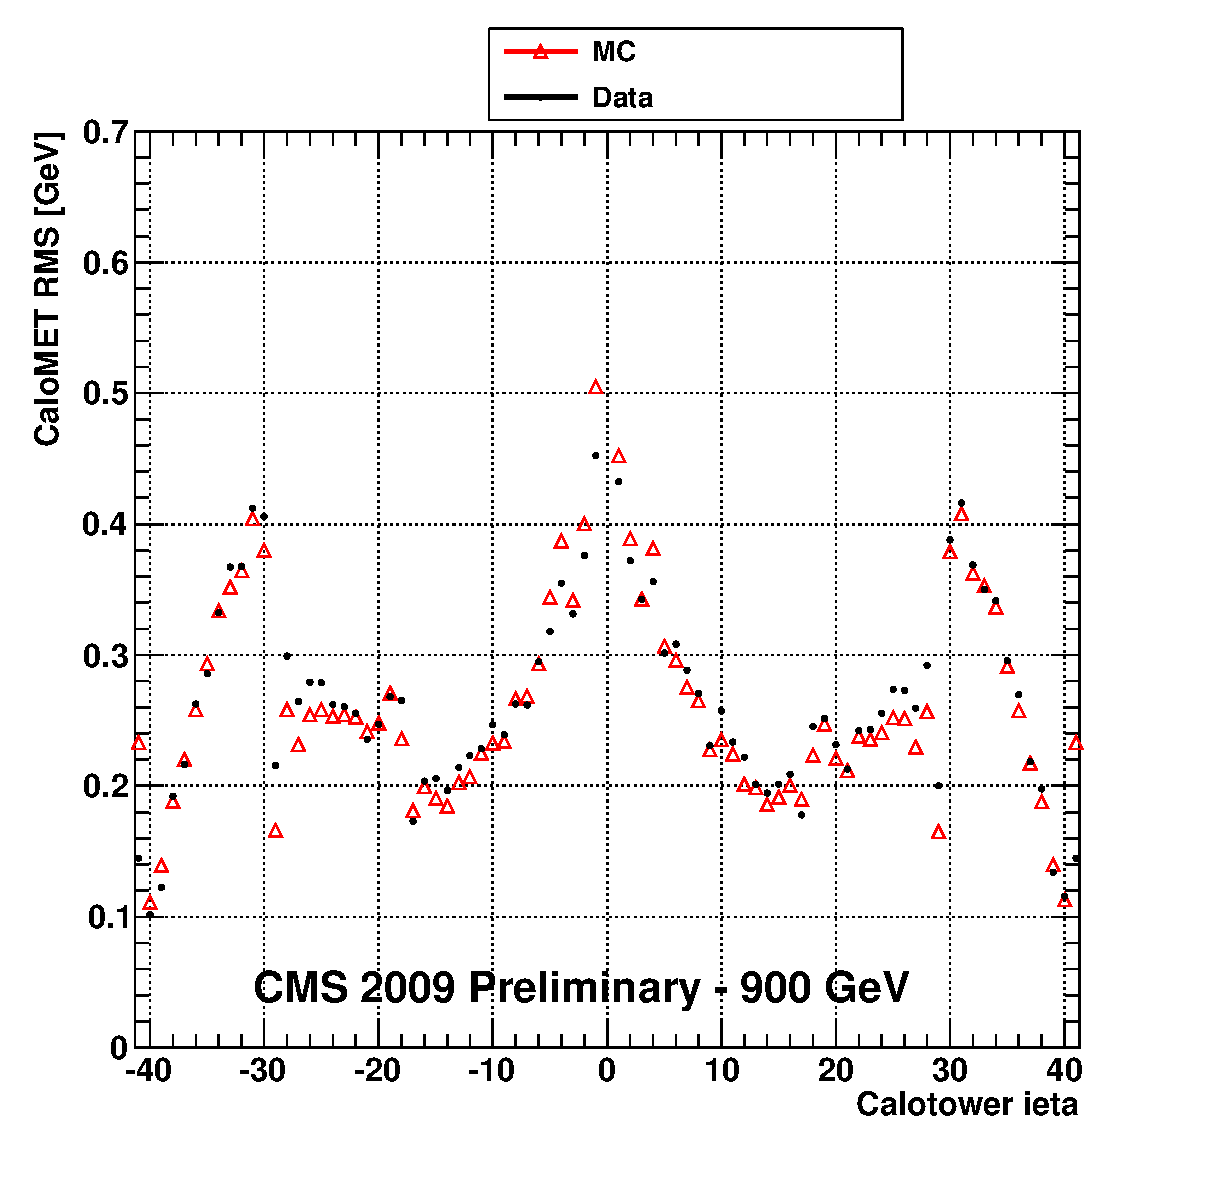
\includegraphics[width=0.5\textwidth]{plots_DataVsMC_MB_900GeV/g_calometPtRMS_vs_ieta_900.eps} \\
 \end{tabular}
 \caption{\small Comparison of the $\etmiss$ Mean vs. i$\eta$ of calotowers and $\etmiss$ RMS vs. i$\eta$ of calotowers between 
          Monte Carlo and data at $900$ GeV.\label{fig:MET_MeanRMS_vs_ieta_900}}
\end{figure}

\begin{figure}[h!]
 \centering
 \begin{tabular}{ll}
  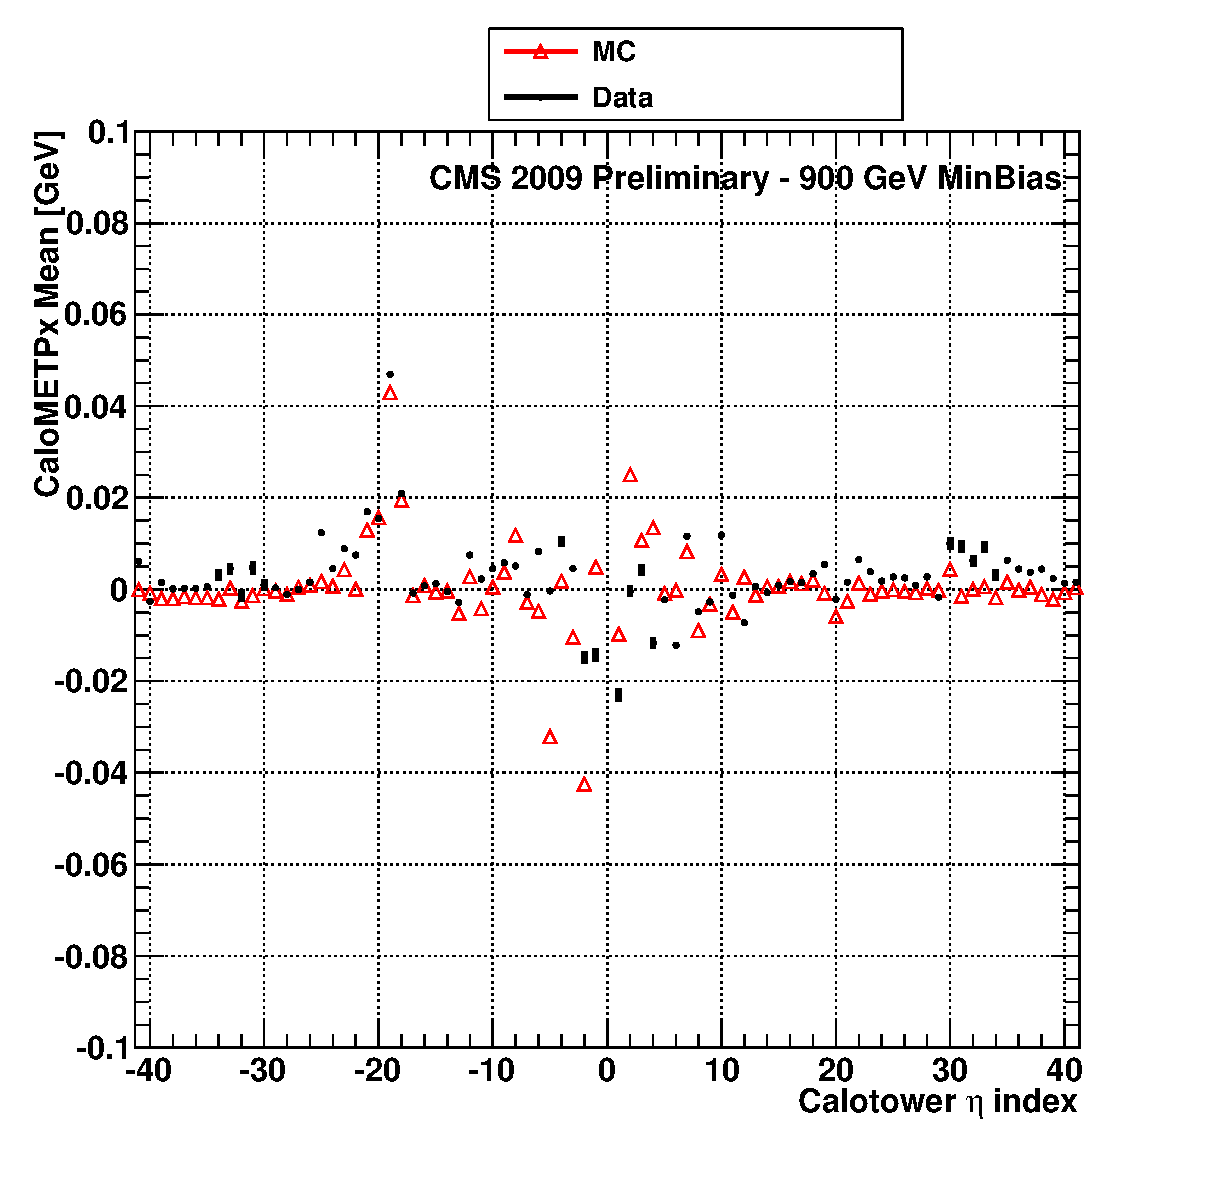
\includegraphics[width=0.5\textwidth]{plots_DataVsMC_MB_900GeV/g_calometPxMean_vs_ieta_900.eps} &
  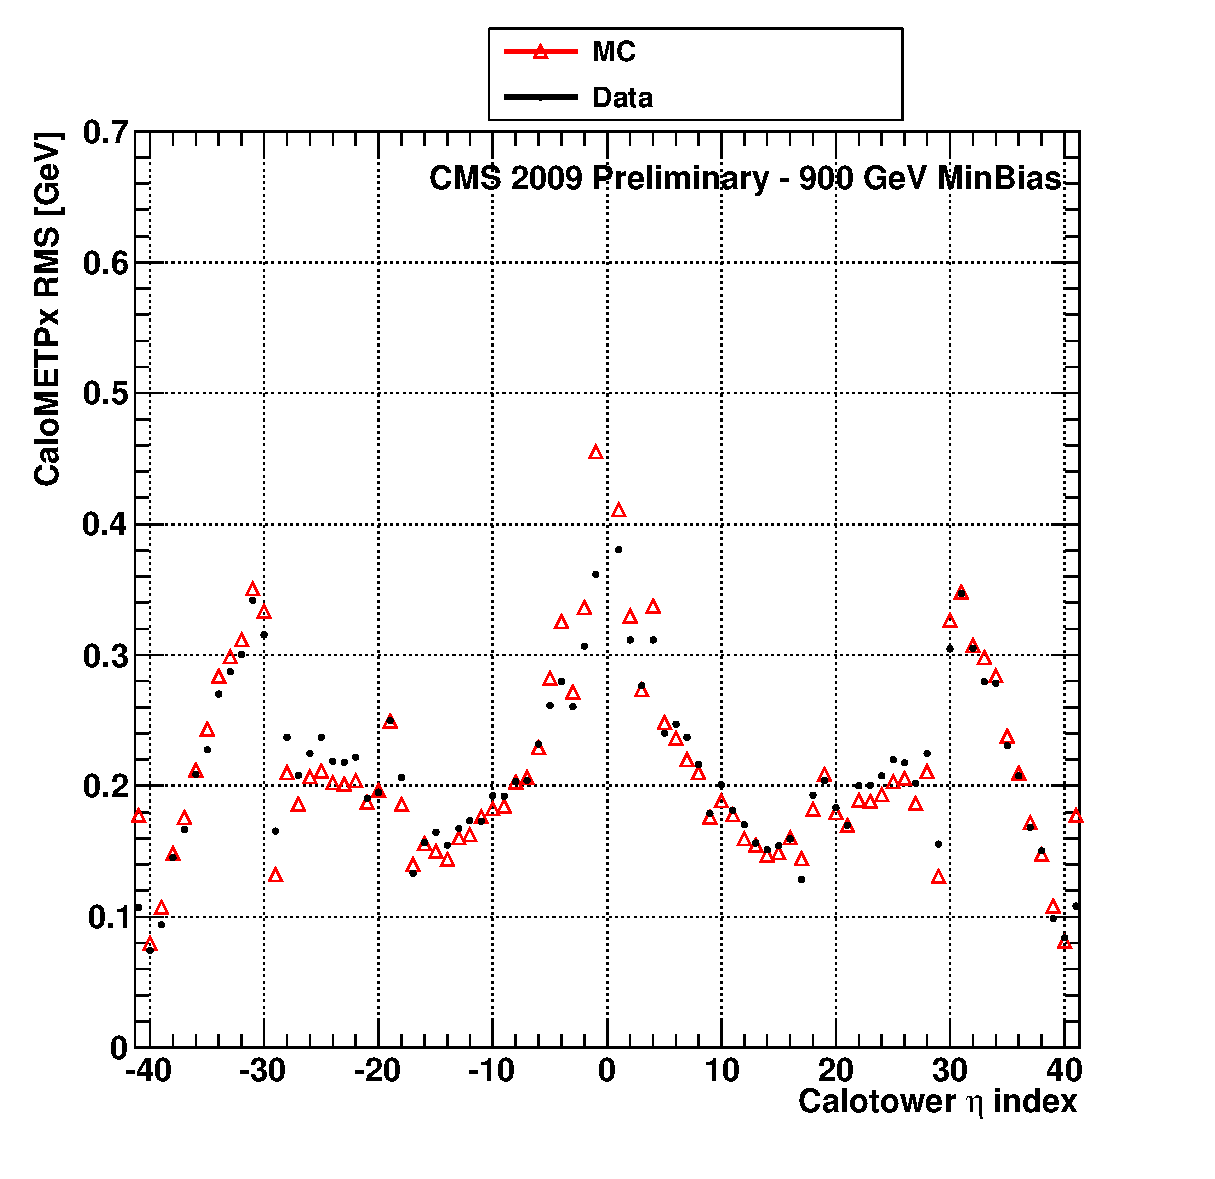
\includegraphics[width=0.5\textwidth]{plots_DataVsMC_MB_900GeV/g_calometPxRMS_vs_ieta_900.eps} \\
 \end{tabular}
 \caption{\small Comparison of the $\exmiss$ Mean vs. i$\eta$ of calotowers and $\exmiss$ RMS vs. i$\eta$ of calotowers between 
          Monte Carlo and data at $900$ GeV.\label{fig:METx_MeanRMS_vs_ieta_900}}
\end{figure}

\begin{figure}[h!]
 \centering
 \begin{tabular}{ll}
  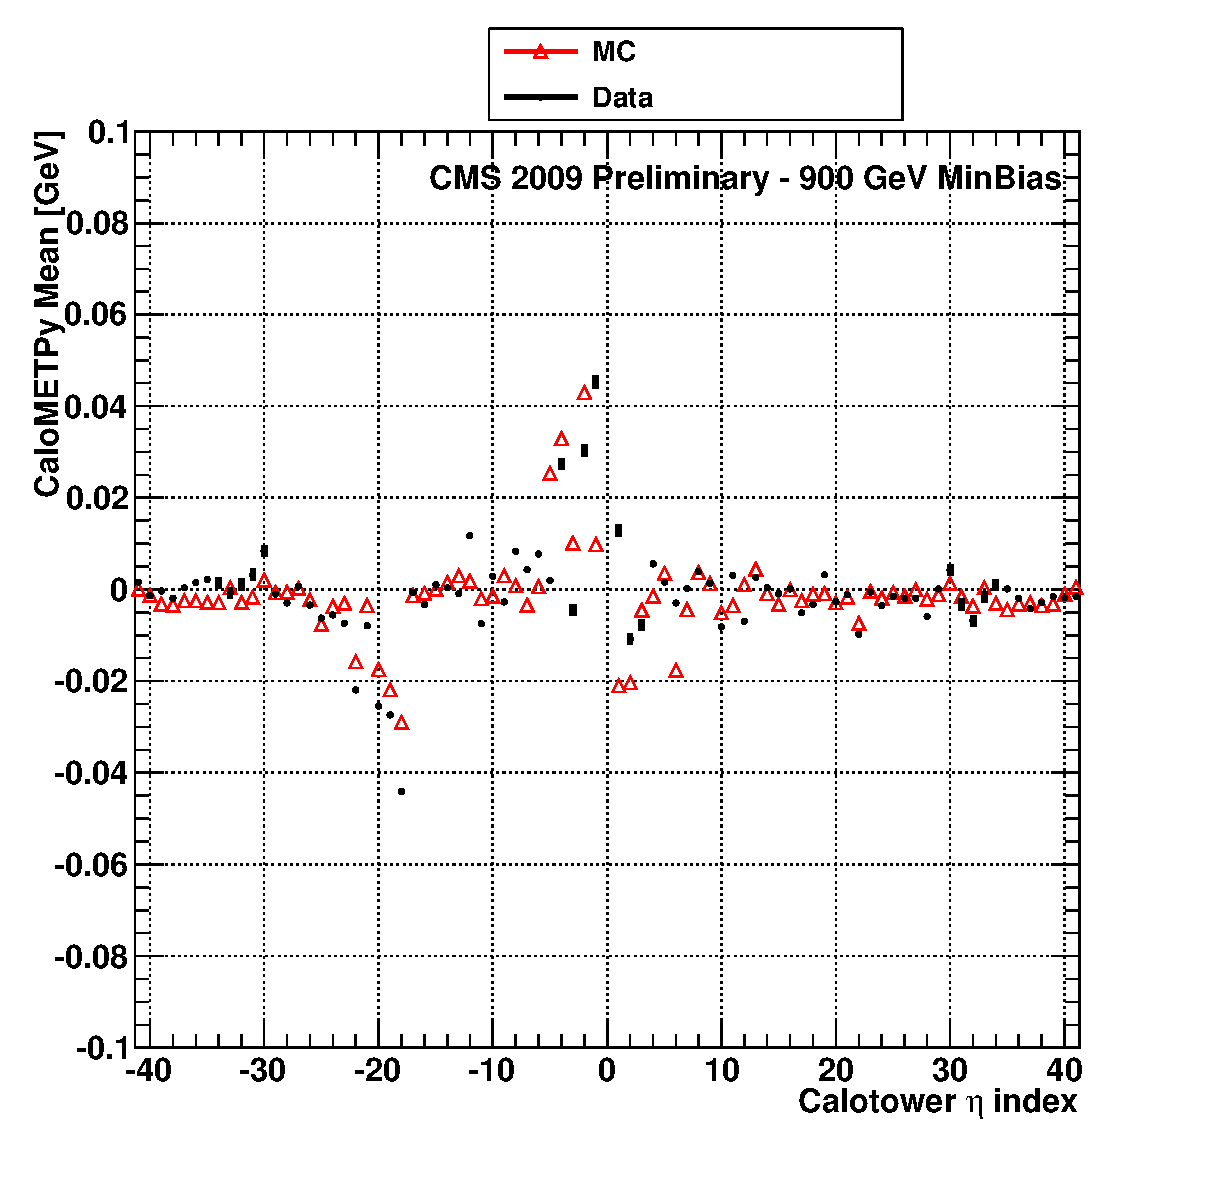
\includegraphics[width=0.5\textwidth]{plots_DataVsMC_MB_900GeV/g_calometPyMean_vs_ieta_900.eps} &
  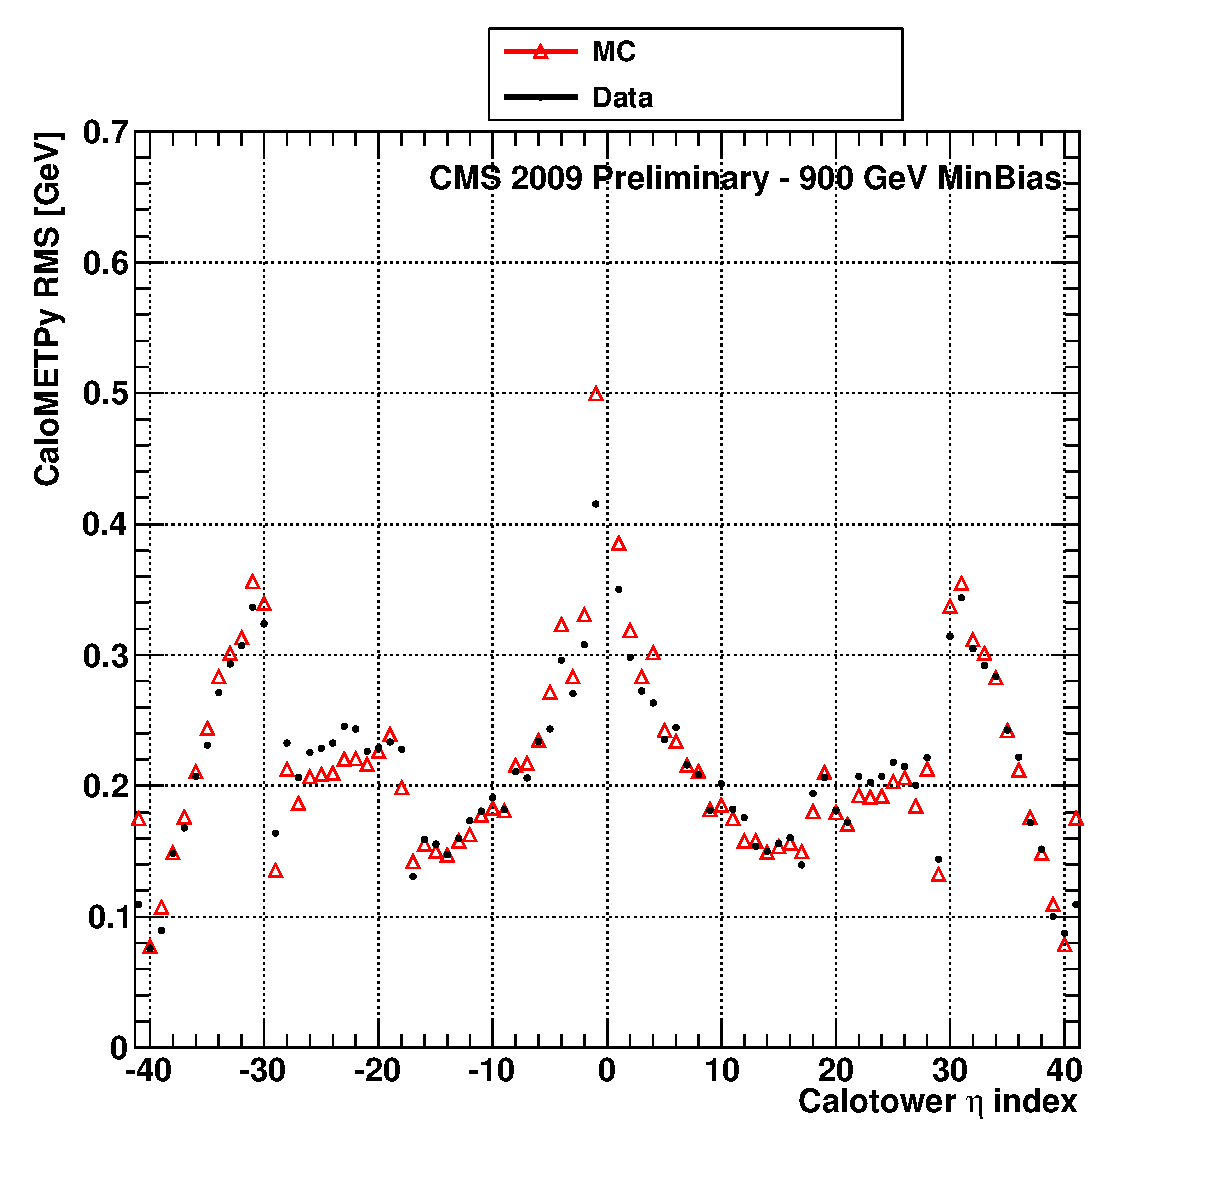
\includegraphics[width=0.5\textwidth]{plots_DataVsMC_MB_900GeV/g_calometPyRMS_vs_ieta_900.eps} \\
 \end{tabular}
 \caption{\small Comparison of the $\eymiss$ Mean vs. i$\eta$ of calotowers and $\eymiss$ RMS vs. i$\eta$ of calotowers between 
          Monte Carlo and data at $900$ GeV.\label{fig:METy_MeanRMS_vs_ieta_900}}
\end{figure}

\clearpage
